\documentclass[twoside]{book}

% Packages required by doxygen
\usepackage{calc}
\usepackage{doxygen}
\usepackage{graphicx}
\usepackage[utf8]{inputenc}
\usepackage{makeidx}
\usepackage{multicol}
\usepackage{multirow}
\usepackage{textcomp}
\usepackage[table]{xcolor}

% Font selection
\usepackage[T1]{fontenc}
\usepackage{mathptmx}
\usepackage[scaled=.90]{helvet}
\usepackage{courier}
\usepackage{amssymb}
\usepackage{sectsty}
\renewcommand{\familydefault}{\sfdefault}
\allsectionsfont{%
  \fontseries{bc}\selectfont%
  \color{darkgray}%
}
\renewcommand{\DoxyLabelFont}{%
  \fontseries{bc}\selectfont%
  \color{darkgray}%
}

% Page & text layout
\usepackage{geometry}
\geometry{%
  a4paper,%
  top=2.5cm,%
  bottom=2.5cm,%
  left=2.5cm,%
  right=2.5cm%
}
\tolerance=750
\hfuzz=15pt
\hbadness=750
\setlength{\emergencystretch}{15pt}
\setlength{\parindent}{0cm}
\setlength{\parskip}{0.2cm}
\makeatletter
\renewcommand{\paragraph}{%
  \@startsection{paragraph}{4}{0ex}{-1.0ex}{1.0ex}{%
    \normalfont\normalsize\bfseries\SS@parafont%
  }%
}
\renewcommand{\subparagraph}{%
  \@startsection{subparagraph}{5}{0ex}{-1.0ex}{1.0ex}{%
    \normalfont\normalsize\bfseries\SS@subparafont%
  }%
}
\makeatother

% Headers & footers
\usepackage{fancyhdr}
\pagestyle{fancyplain}
\fancyhead[LE]{\fancyplain{}{\bfseries\thepage}}
\fancyhead[CE]{\fancyplain{}{}}
\fancyhead[RE]{\fancyplain{}{\bfseries\leftmark}}
\fancyhead[LO]{\fancyplain{}{\bfseries\rightmark}}
\fancyhead[CO]{\fancyplain{}{}}
\fancyhead[RO]{\fancyplain{}{\bfseries\thepage}}
\fancyfoot[LE]{\fancyplain{}{}}
\fancyfoot[CE]{\fancyplain{}{}}
\fancyfoot[RE]{\fancyplain{}{\bfseries\scriptsize Generated on Wed Dec 4 2013 22\-:23\-:41 for Tailored Travels by Doxygen }}
\fancyfoot[LO]{\fancyplain{}{\bfseries\scriptsize Generated on Wed Dec 4 2013 22\-:23\-:41 for Tailored Travels by Doxygen }}
\fancyfoot[CO]{\fancyplain{}{}}
\fancyfoot[RO]{\fancyplain{}{}}
\renewcommand{\footrulewidth}{0.4pt}
\renewcommand{\chaptermark}[1]{%
  \markboth{#1}{}%
}
\renewcommand{\sectionmark}[1]{%
  \markright{\thesection\ #1}%
}

% Indices & bibliography
\usepackage{natbib}
\usepackage[titles]{tocloft}
\setcounter{tocdepth}{3}
\setcounter{secnumdepth}{5}
\makeindex

% Hyperlinks (required, but should be loaded last)
\usepackage{ifpdf}
\ifpdf
  \usepackage[pdftex,pagebackref=true]{hyperref}
\else
  \usepackage[ps2pdf,pagebackref=true]{hyperref}
\fi
\hypersetup{%
  colorlinks=true,%
  linkcolor=blue,%
  citecolor=blue,%
  unicode%
}

% Custom commands
\newcommand{\clearemptydoublepage}{%
  \newpage{\pagestyle{empty}\cleardoublepage}%
}


%===== C O N T E N T S =====

\begin{document}

% Titlepage & ToC
\hypersetup{pageanchor=false}
\pagenumbering{roman}
\begin{titlepage}
\vspace*{7cm}
\begin{center}%
{\Large Tailored Travels }\\
\vspace*{1cm}
{\large Generated by Doxygen 1.8.5}\\
\vspace*{0.5cm}
{\small Wed Dec 4 2013 22:23:41}\\
\end{center}
\end{titlepage}
\clearemptydoublepage
\tableofcontents
\clearemptydoublepage
\pagenumbering{arabic}
\hypersetup{pageanchor=true}

%--- Begin generated contents ---
\chapter{Namespace Index}
\section{Packages}
Here are the packages with brief descriptions (if available)\-:\begin{DoxyCompactList}
\item\contentsline{section}{\hyperlink{namespacecom}{com} }{\pageref{namespacecom}}{}
\item\contentsline{section}{\hyperlink{namespacecom_1_1twix}{com.\-twix} }{\pageref{namespacecom_1_1twix}}{}
\item\contentsline{section}{\hyperlink{namespacecom_1_1twix_1_1init}{com.\-twix.\-init} }{\pageref{namespacecom_1_1twix_1_1init}}{}
\item\contentsline{section}{\hyperlink{namespacecom_1_1twix_1_1tailoredtravels}{com.\-twix.\-tailoredtravels} }{\pageref{namespacecom_1_1twix_1_1tailoredtravels}}{}
\end{DoxyCompactList}

\chapter{Hierarchical Index}
\section{Class Hierarchy}
This inheritance list is sorted roughly, but not completely, alphabetically\-:\begin{DoxyCompactList}
\item \contentsline{section}{com.\-twix.\-tailoredtravels.\-Client}{\pageref{classcom_1_1twix_1_1tailoredtravels_1_1_client}}{}
\item \contentsline{section}{com.\-twix.\-tailoredtravels.\-Database\-Manager}{\pageref{classcom_1_1twix_1_1tailoredtravels_1_1_database_manager}}{}
\item \contentsline{section}{com.\-twix.\-tailoredtravels.\-Dist\-Calc\-Driver}{\pageref{classcom_1_1twix_1_1tailoredtravels_1_1_dist_calc_driver}}{}
\item \contentsline{section}{com.\-twix.\-tailoredtravels.\-Google\-Earth\-Manager}{\pageref{classcom_1_1twix_1_1tailoredtravels_1_1_google_earth_manager}}{}
\item \contentsline{section}{com.\-twix.\-tailoredtravels.\-Google\-Earth\-Path}{\pageref{classcom_1_1twix_1_1tailoredtravels_1_1_google_earth_path}}{}
\item \contentsline{section}{com.\-twix.\-init.\-Init\-Database}{\pageref{classcom_1_1twix_1_1init_1_1_init_database}}{}
\item \contentsline{section}{com.\-twix.\-tailoredtravels.\-Lat\-Long\-Pair}{\pageref{classcom_1_1twix_1_1tailoredtravels_1_1_lat_long_pair}}{}
\item Runnable\begin{DoxyCompactList}
\item \contentsline{section}{com.\-twix.\-tailoredtravels.\-Progress\-Bar}{\pageref{classcom_1_1twix_1_1tailoredtravels_1_1_progress_bar}}{}
\end{DoxyCompactList}
\item \contentsline{section}{com.\-twix.\-tailoredtravels.\-Waypoint}{\pageref{classcom_1_1twix_1_1tailoredtravels_1_1_waypoint}}{}
\item J\-Panel\begin{DoxyCompactList}
\item \contentsline{section}{com.\-twix.\-tailoredtravels.\-Menu\-Panel}{\pageref{classcom_1_1twix_1_1tailoredtravels_1_1_menu_panel}}{}
\item \contentsline{section}{com.\-twix.\-tailoredtravels.\-Progress\-Bar}{\pageref{classcom_1_1twix_1_1tailoredtravels_1_1_progress_bar}}{}
\end{DoxyCompactList}
\end{DoxyCompactList}

\chapter{Class Index}
\section{Class List}
Here are the classes, structs, unions and interfaces with brief descriptions\-:\begin{DoxyCompactList}
\item\contentsline{section}{\hyperlink{classcom_1_1twix_1_1tailoredtravels_1_1_client}{com.\-twix.\-tailoredtravels.\-Client} }{\pageref{classcom_1_1twix_1_1tailoredtravels_1_1_client}}{}
\item\contentsline{section}{\hyperlink{classcom_1_1twix_1_1tailoredtravels_1_1_database_manager}{com.\-twix.\-tailoredtravels.\-Database\-Manager} }{\pageref{classcom_1_1twix_1_1tailoredtravels_1_1_database_manager}}{}
\item\contentsline{section}{\hyperlink{classcom_1_1twix_1_1tailoredtravels_1_1_dist_calc_driver}{com.\-twix.\-tailoredtravels.\-Dist\-Calc\-Driver} }{\pageref{classcom_1_1twix_1_1tailoredtravels_1_1_dist_calc_driver}}{}
\item\contentsline{section}{\hyperlink{classcom_1_1twix_1_1tailoredtravels_1_1_google_earth_manager}{com.\-twix.\-tailoredtravels.\-Google\-Earth\-Manager} }{\pageref{classcom_1_1twix_1_1tailoredtravels_1_1_google_earth_manager}}{}
\item\contentsline{section}{\hyperlink{classcom_1_1twix_1_1tailoredtravels_1_1_google_earth_path}{com.\-twix.\-tailoredtravels.\-Google\-Earth\-Path} }{\pageref{classcom_1_1twix_1_1tailoredtravels_1_1_google_earth_path}}{}
\item\contentsline{section}{\hyperlink{classcom_1_1twix_1_1init_1_1_init_database}{com.\-twix.\-init.\-Init\-Database} }{\pageref{classcom_1_1twix_1_1init_1_1_init_database}}{}
\item\contentsline{section}{\hyperlink{classcom_1_1twix_1_1tailoredtravels_1_1_lat_long_pair}{com.\-twix.\-tailoredtravels.\-Lat\-Long\-Pair} }{\pageref{classcom_1_1twix_1_1tailoredtravels_1_1_lat_long_pair}}{}
\item\contentsline{section}{\hyperlink{classcom_1_1twix_1_1tailoredtravels_1_1_menu_panel}{com.\-twix.\-tailoredtravels.\-Menu\-Panel} }{\pageref{classcom_1_1twix_1_1tailoredtravels_1_1_menu_panel}}{}
\item\contentsline{section}{\hyperlink{classcom_1_1twix_1_1tailoredtravels_1_1_progress_bar}{com.\-twix.\-tailoredtravels.\-Progress\-Bar} }{\pageref{classcom_1_1twix_1_1tailoredtravels_1_1_progress_bar}}{}
\item\contentsline{section}{\hyperlink{classcom_1_1twix_1_1tailoredtravels_1_1_waypoint}{com.\-twix.\-tailoredtravels.\-Waypoint} }{\pageref{classcom_1_1twix_1_1tailoredtravels_1_1_waypoint}}{}
\end{DoxyCompactList}

\chapter{File Index}
\section{File List}
Here is a list of all files with brief descriptions\-:\begin{DoxyCompactList}
\item\contentsline{section}{C\-:/\-Users/\-Justin/workspace/\-Tailored Travels/src/com/twix/init/\hyperlink{_init_database_8java}{Init\-Database.\-java} }{\pageref{_init_database_8java}}{}
\item\contentsline{section}{C\-:/\-Users/\-Justin/workspace/\-Tailored Travels/src/com/twix/tailoredtravels/\hyperlink{_client_8java}{Client.\-java} }{\pageref{_client_8java}}{}
\item\contentsline{section}{C\-:/\-Users/\-Justin/workspace/\-Tailored Travels/src/com/twix/tailoredtravels/\hyperlink{_database_manager_8java}{Database\-Manager.\-java} }{\pageref{_database_manager_8java}}{}
\item\contentsline{section}{C\-:/\-Users/\-Justin/workspace/\-Tailored Travels/src/com/twix/tailoredtravels/\hyperlink{_dist_calc_driver_8java}{Dist\-Calc\-Driver.\-java} }{\pageref{_dist_calc_driver_8java}}{}
\item\contentsline{section}{C\-:/\-Users/\-Justin/workspace/\-Tailored Travels/src/com/twix/tailoredtravels/\hyperlink{_google_earth_manager_8java}{Google\-Earth\-Manager.\-java} }{\pageref{_google_earth_manager_8java}}{}
\item\contentsline{section}{C\-:/\-Users/\-Justin/workspace/\-Tailored Travels/src/com/twix/tailoredtravels/\hyperlink{_google_earth_path_8java}{Google\-Earth\-Path.\-java} }{\pageref{_google_earth_path_8java}}{}
\item\contentsline{section}{C\-:/\-Users/\-Justin/workspace/\-Tailored Travels/src/com/twix/tailoredtravels/\hyperlink{_lat_long_pair_8java}{Lat\-Long\-Pair.\-java} }{\pageref{_lat_long_pair_8java}}{}
\item\contentsline{section}{C\-:/\-Users/\-Justin/workspace/\-Tailored Travels/src/com/twix/tailoredtravels/\hyperlink{_menu_panel_8java}{Menu\-Panel.\-java} }{\pageref{_menu_panel_8java}}{}
\item\contentsline{section}{C\-:/\-Users/\-Justin/workspace/\-Tailored Travels/src/com/twix/tailoredtravels/\hyperlink{_progress_bar_8java}{Progress\-Bar.\-java} }{\pageref{_progress_bar_8java}}{}
\item\contentsline{section}{C\-:/\-Users/\-Justin/workspace/\-Tailored Travels/src/com/twix/tailoredtravels/\hyperlink{_waypoint_8java}{Waypoint.\-java} }{\pageref{_waypoint_8java}}{}
\end{DoxyCompactList}

\chapter{Namespace Documentation}
\hypertarget{namespacecom}{\section{Package com}
\label{namespacecom}\index{com@{com}}
}
\subsection*{Packages}
\begin{DoxyCompactItemize}
\item 
package \hyperlink{namespacecom_1_1twix}{twix}
\end{DoxyCompactItemize}

\hypertarget{namespacecom_1_1twix}{\section{Package com.\-twix}
\label{namespacecom_1_1twix}\index{com.\-twix@{com.\-twix}}
}
\subsection*{Packages}
\begin{DoxyCompactItemize}
\item 
package \hyperlink{namespacecom_1_1twix_1_1init}{init}
\item 
package \hyperlink{namespacecom_1_1twix_1_1tailoredtravels}{tailoredtravels}
\end{DoxyCompactItemize}

\hypertarget{namespacecom_1_1twix_1_1init}{\section{Package com.\-twix.\-init}
\label{namespacecom_1_1twix_1_1init}\index{com.\-twix.\-init@{com.\-twix.\-init}}
}
\subsection*{Classes}
\begin{DoxyCompactItemize}
\item 
class \hyperlink{classcom_1_1twix_1_1init_1_1_init_database}{Init\-Database}
\end{DoxyCompactItemize}

\hypertarget{namespacecom_1_1twix_1_1tailoredtravels}{\section{Package com.\-twix.\-tailoredtravels}
\label{namespacecom_1_1twix_1_1tailoredtravels}\index{com.\-twix.\-tailoredtravels@{com.\-twix.\-tailoredtravels}}
}
\subsection*{Classes}
\begin{DoxyCompactItemize}
\item 
class \hyperlink{classcom_1_1twix_1_1tailoredtravels_1_1_client}{Client}
\item 
class \hyperlink{classcom_1_1twix_1_1tailoredtravels_1_1_database_manager}{Database\-Manager}
\item 
class \hyperlink{classcom_1_1twix_1_1tailoredtravels_1_1_dist_calc_driver}{Dist\-Calc\-Driver}
\item 
class \hyperlink{classcom_1_1twix_1_1tailoredtravels_1_1_google_earth_manager}{Google\-Earth\-Manager}
\item 
class \hyperlink{classcom_1_1twix_1_1tailoredtravels_1_1_google_earth_path}{Google\-Earth\-Path}
\item 
class \hyperlink{classcom_1_1twix_1_1tailoredtravels_1_1_lat_long_pair}{Lat\-Long\-Pair}
\item 
class \hyperlink{classcom_1_1twix_1_1tailoredtravels_1_1_menu_panel}{Menu\-Panel}
\item 
class \hyperlink{classcom_1_1twix_1_1tailoredtravels_1_1_messages}{Messages}
\item 
class \hyperlink{classcom_1_1twix_1_1tailoredtravels_1_1_progress_bar}{Progress\-Bar}
\item 
class \hyperlink{classcom_1_1twix_1_1tailoredtravels_1_1_waypoint}{Waypoint}
\end{DoxyCompactItemize}


\subsection{Detailed Description}
Where the program starts. Users are prompted for user names and passwords then Google Earth opens.

\begin{DoxyAuthor}{Author}
Christopher Pagan 
\end{DoxyAuthor}
\begin{DoxyVersion}{Version}
1.\-0
\end{DoxyVersion}
A class used in handling all calls to Google Earth and all K\-M\-L manipulation.

\begin{DoxyAuthor}{Author}
Stephen Moore
\end{DoxyAuthor}
A class used to maintain an ordered list of Waypoints to send to Google Earth.

\begin{DoxyAuthor}{Author}
Stephen Moore
\end{DoxyAuthor}
Panel containing the main menu and most administrator and user functions. Only logged in users will be able to access this window.

\begin{DoxyAuthor}{Author}
Christopher Pagan 
\end{DoxyAuthor}
\begin{DoxyVersion}{Version}
1.\-0
\end{DoxyVersion}
Progress bad runnable J\-Panel

\begin{DoxyAuthor}{Author}
Keith Cheng with Christopher Pagan 
\end{DoxyAuthor}

\chapter{Class Documentation}
\hypertarget{classcom_1_1twix_1_1tailoredtravels_1_1_client}{\section{com.\-twix.\-tailoredtravels.\-Client Class Reference}
\label{classcom_1_1twix_1_1tailoredtravels_1_1_client}\index{com.\-twix.\-tailoredtravels.\-Client@{com.\-twix.\-tailoredtravels.\-Client}}
}
\subsection*{Static Public Member Functions}
\begin{DoxyCompactItemize}
\item 
static void \hyperlink{classcom_1_1twix_1_1tailoredtravels_1_1_client_a781f21b89856adb998c7929b4221923e}{main} (String\mbox{[}$\,$\mbox{]} args)
\item 
static void \hyperlink{classcom_1_1twix_1_1tailoredtravels_1_1_client_a5beadc73343776db6ad205390c38f0a9}{show\-Main\-Menu} (\hyperlink{classcom_1_1twix_1_1tailoredtravels_1_1_database_manager}{Database\-Manager} dbm, String user\-Name, boolean admin)
\end{DoxyCompactItemize}


\subsection{Member Function Documentation}
\hypertarget{classcom_1_1twix_1_1tailoredtravels_1_1_client_a781f21b89856adb998c7929b4221923e}{\index{com\-::twix\-::tailoredtravels\-::\-Client@{com\-::twix\-::tailoredtravels\-::\-Client}!main@{main}}
\index{main@{main}!com::twix::tailoredtravels::Client@{com\-::twix\-::tailoredtravels\-::\-Client}}
\subsubsection[{main}]{\setlength{\rightskip}{0pt plus 5cm}static void com.\-twix.\-tailoredtravels.\-Client.\-main (
\begin{DoxyParamCaption}
\item[{String\mbox{[}$\,$\mbox{]}}]{args}
\end{DoxyParamCaption}
)\hspace{0.3cm}{\ttfamily [static]}}}\label{classcom_1_1twix_1_1tailoredtravels_1_1_client_a781f21b89856adb998c7929b4221923e}
Main method -\/ Creates login panel, handles login information


\begin{DoxyParams}{Parameters}
{\em args} & no arguments used \\
\hline
\end{DoxyParams}

\begin{DoxyExceptions}{Exceptions}
{\em Unsupported\-Look\-And\-Feel\-Exception} & \\
\hline
{\em Illegal\-Access\-Exception} & \\
\hline
{\em Instantiation\-Exception} & \\
\hline
{\em Class\-Not\-Found\-Exception} & \\
\hline
\end{DoxyExceptions}
Overwritten method for Action\-Listener class. Verifies the user is authorized to use the system.


\begin{DoxyParams}{Parameters}
{\em e} & An Action\-Event is created when the user clicks the login button\\
\hline
\end{DoxyParams}
\hypertarget{classcom_1_1twix_1_1tailoredtravels_1_1_client_a5beadc73343776db6ad205390c38f0a9}{\index{com\-::twix\-::tailoredtravels\-::\-Client@{com\-::twix\-::tailoredtravels\-::\-Client}!show\-Main\-Menu@{show\-Main\-Menu}}
\index{show\-Main\-Menu@{show\-Main\-Menu}!com::twix::tailoredtravels::Client@{com\-::twix\-::tailoredtravels\-::\-Client}}
\subsubsection[{show\-Main\-Menu}]{\setlength{\rightskip}{0pt plus 5cm}static void com.\-twix.\-tailoredtravels.\-Client.\-show\-Main\-Menu (
\begin{DoxyParamCaption}
\item[{{\bf Database\-Manager}}]{dbm, }
\item[{String}]{user\-Name, }
\item[{boolean}]{admin}
\end{DoxyParamCaption}
)\hspace{0.3cm}{\ttfamily [static]}}}\label{classcom_1_1twix_1_1tailoredtravels_1_1_client_a5beadc73343776db6ad205390c38f0a9}
Opens up the main menu screen


\begin{DoxyParams}{Parameters}
{\em dbm} & the dbm that contains user and location information \\
\hline
{\em user\-Name} & the user's username \\
\hline
{\em admin} & whether or not a user is an administrator \\
\hline
\end{DoxyParams}


The documentation for this class was generated from the following file\-:\begin{DoxyCompactItemize}
\item 
C\-:/\-Users/\-Justin/workspace/\-Tailored Travels/src/com/twix/tailoredtravels/\hyperlink{_client_8java}{Client.\-java}\end{DoxyCompactItemize}

\hypertarget{classcom_1_1twix_1_1tailoredtravels_1_1_database_manager}{\section{com.\-twix.\-tailoredtravels.\-Database\-Manager Class Reference}
\label{classcom_1_1twix_1_1tailoredtravels_1_1_database_manager}\index{com.\-twix.\-tailoredtravels.\-Database\-Manager@{com.\-twix.\-tailoredtravels.\-Database\-Manager}}
}
\subsection*{Public Member Functions}
\begin{DoxyCompactItemize}
\item 
\hyperlink{classcom_1_1twix_1_1tailoredtravels_1_1_database_manager_a5fd81387462021f3a2c234596d7e669f}{Database\-Manager} ()  throws Class\-Not\-Found\-Exception, S\-Q\-L\-Exception 	
\item 
boolean \hyperlink{classcom_1_1twix_1_1tailoredtravels_1_1_database_manager_a7ad514c70febbb99b14d8a4dab1b24a6}{login} (String name, String password)  throws S\-Q\-L\-Exception 	
\item 
void \hyperlink{classcom_1_1twix_1_1tailoredtravels_1_1_database_manager_a3fe7ef841c1340941920745cc00a39ab}{logout} ()
\item 
boolean \hyperlink{classcom_1_1twix_1_1tailoredtravels_1_1_database_manager_ab60c1da42acf1d6ecc8955aa58da3803}{add\-User} (String name, String password, boolean is\-Admin)  throws S\-Q\-L\-Exception 	
\item 
boolean \hyperlink{classcom_1_1twix_1_1tailoredtravels_1_1_database_manager_a19c56c261a486a909936cf7c97334360}{add\-Location} (float latitude, float longitude, String name, String description)  throws S\-Q\-L\-Exception 	
\item 
boolean \hyperlink{classcom_1_1twix_1_1tailoredtravels_1_1_database_manager_a73d155c07d2ed41e8c596323184da135}{remove\-User} (String name)  throws S\-Q\-L\-Exception 	
\item 
boolean \hyperlink{classcom_1_1twix_1_1tailoredtravels_1_1_database_manager_ac60ff9d81a074ef84eb0f6ced1fa7fde}{remove\-Location} (String name)  throws S\-Q\-L\-Exception 	
\item 
boolean \hyperlink{classcom_1_1twix_1_1tailoredtravels_1_1_database_manager_a4c8078e19441474ebb02fd67dfe9d3b4}{set\-Waypoint\-Name} (String old\-Name, String new\-Name)  throws S\-Q\-L\-Exception 	
\item 
boolean \hyperlink{classcom_1_1twix_1_1tailoredtravels_1_1_database_manager_aa8c98a1bfb16ebdbd8d3eeb6e9d80a73}{set\-Waypoint\-Description} (String old\-Description, String new\-Description)  throws S\-Q\-L\-Exception 	
\item 
boolean \hyperlink{classcom_1_1twix_1_1tailoredtravels_1_1_database_manager_a0b8a3295e6857761b89a8db4d048d5a4}{set\-Waypoint\-Lat\-Long} (String name, float new\-Lat, float new\-Long)  throws S\-Q\-L\-Exception 	
\item 
boolean \hyperlink{classcom_1_1twix_1_1tailoredtravels_1_1_database_manager_a2ccf63adbc938676d9bafbf43667261a}{is\-User\-Admin} ()
\item 
Linked\-List$<$ \hyperlink{classcom_1_1twix_1_1tailoredtravels_1_1_waypoint}{Waypoint} $>$ \hyperlink{classcom_1_1twix_1_1tailoredtravels_1_1_database_manager_a4e594f8a6f845de1fe5ab29e5430ba9e}{get\-Waypoints} ()  throws S\-Q\-L\-Exception 	
\item 
void \hyperlink{classcom_1_1twix_1_1tailoredtravels_1_1_database_manager_ac69a6164612bb086c72c54440d32f3de}{print\-Waypoints} ()
\end{DoxyCompactItemize}


\subsection{Detailed Description}
There M\-U\-S\-T be a derby embeddeddriver loaded in plugins The database must exist 

\subsection{Constructor \& Destructor Documentation}
\hypertarget{classcom_1_1twix_1_1tailoredtravels_1_1_database_manager_a5fd81387462021f3a2c234596d7e669f}{\index{com\-::twix\-::tailoredtravels\-::\-Database\-Manager@{com\-::twix\-::tailoredtravels\-::\-Database\-Manager}!Database\-Manager@{Database\-Manager}}
\index{Database\-Manager@{Database\-Manager}!com::twix::tailoredtravels::DatabaseManager@{com\-::twix\-::tailoredtravels\-::\-Database\-Manager}}
\subsubsection[{Database\-Manager}]{\setlength{\rightskip}{0pt plus 5cm}com.\-twix.\-tailoredtravels.\-Database\-Manager.\-Database\-Manager (
\begin{DoxyParamCaption}
{}
\end{DoxyParamCaption}
) throws Class\-Not\-Found\-Exception, S\-Q\-L\-Exception}}\label{classcom_1_1twix_1_1tailoredtravels_1_1_database_manager_a5fd81387462021f3a2c234596d7e669f}
Constructor that starts this file reader reads the location file and user file to have data

precondition\-: org.\-apache.\-derby.\-jdbc.\-Embedded\-Driver must exist in eclipse plugin postcondition\-: sets current\-User to 0 to mean no user at this time sets login to false


\begin{DoxyExceptions}{Exceptions}
{\em Class\-Not\-Fount\-Exception} & \\
\hline
{\em S\-Q\-L\-Exception} & \\
\hline
\end{DoxyExceptions}


\subsection{Member Function Documentation}
\hypertarget{classcom_1_1twix_1_1tailoredtravels_1_1_database_manager_a19c56c261a486a909936cf7c97334360}{\index{com\-::twix\-::tailoredtravels\-::\-Database\-Manager@{com\-::twix\-::tailoredtravels\-::\-Database\-Manager}!add\-Location@{add\-Location}}
\index{add\-Location@{add\-Location}!com::twix::tailoredtravels::DatabaseManager@{com\-::twix\-::tailoredtravels\-::\-Database\-Manager}}
\subsubsection[{add\-Location}]{\setlength{\rightskip}{0pt plus 5cm}boolean com.\-twix.\-tailoredtravels.\-Database\-Manager.\-add\-Location (
\begin{DoxyParamCaption}
\item[{float}]{latitude, }
\item[{float}]{longitude, }
\item[{String}]{name, }
\item[{String}]{description}
\end{DoxyParamCaption}
) throws S\-Q\-L\-Exception}}\label{classcom_1_1twix_1_1tailoredtravels_1_1_database_manager_a19c56c261a486a909936cf7c97334360}
add new location to file and update the location file


\begin{DoxyParams}{Parameters}
{\em latitude} & \\
\hline
{\em longitude} & \\
\hline
{\em name} & of location \\
\hline
{\em description} & for location\\
\hline
\end{DoxyParams}
\begin{DoxyReturn}{Returns}
true if the user add a location, false if the user cannot add a location
\end{DoxyReturn}

\begin{DoxyExceptions}{Exceptions}
{\em S\-Q\-L\-Exception} & \\
\hline
\end{DoxyExceptions}
\hypertarget{classcom_1_1twix_1_1tailoredtravels_1_1_database_manager_ab60c1da42acf1d6ecc8955aa58da3803}{\index{com\-::twix\-::tailoredtravels\-::\-Database\-Manager@{com\-::twix\-::tailoredtravels\-::\-Database\-Manager}!add\-User@{add\-User}}
\index{add\-User@{add\-User}!com::twix::tailoredtravels::DatabaseManager@{com\-::twix\-::tailoredtravels\-::\-Database\-Manager}}
\subsubsection[{add\-User}]{\setlength{\rightskip}{0pt plus 5cm}boolean com.\-twix.\-tailoredtravels.\-Database\-Manager.\-add\-User (
\begin{DoxyParamCaption}
\item[{String}]{name, }
\item[{String}]{password, }
\item[{boolean}]{is\-Admin}
\end{DoxyParamCaption}
) throws S\-Q\-L\-Exception}}\label{classcom_1_1twix_1_1tailoredtravels_1_1_database_manager_ab60c1da42acf1d6ecc8955aa58da3803}
add user locations and then update the user table

precondition\-: admin is not null


\begin{DoxyParams}{Parameters}
{\em name} & of user \\
\hline
{\em password} & of user \\
\hline
{\em is\-Admin} & -\/ is the user an admin\\
\hline
\end{DoxyParams}
\begin{DoxyReturn}{Returns}
true
\end{DoxyReturn}

\begin{DoxyExceptions}{Exceptions}
{\em S\-Q\-L\-Exception} & \\
\hline
\end{DoxyExceptions}
\hypertarget{classcom_1_1twix_1_1tailoredtravels_1_1_database_manager_a4e594f8a6f845de1fe5ab29e5430ba9e}{\index{com\-::twix\-::tailoredtravels\-::\-Database\-Manager@{com\-::twix\-::tailoredtravels\-::\-Database\-Manager}!get\-Waypoints@{get\-Waypoints}}
\index{get\-Waypoints@{get\-Waypoints}!com::twix::tailoredtravels::DatabaseManager@{com\-::twix\-::tailoredtravels\-::\-Database\-Manager}}
\subsubsection[{get\-Waypoints}]{\setlength{\rightskip}{0pt plus 5cm}Linked\-List$<${\bf Waypoint}$>$ com.\-twix.\-tailoredtravels.\-Database\-Manager.\-get\-Waypoints (
\begin{DoxyParamCaption}
{}
\end{DoxyParamCaption}
) throws S\-Q\-L\-Exception}}\label{classcom_1_1twix_1_1tailoredtravels_1_1_database_manager_a4e594f8a6f845de1fe5ab29e5430ba9e}
Get and return a Linked\-List containing all waypoints

precondition\-: database exists

\begin{DoxyReturn}{Returns}
linked list of all waypoints
\end{DoxyReturn}

\begin{DoxyExceptions}{Exceptions}
{\em S\-Q\-L\-Exception} & \\
\hline
\end{DoxyExceptions}
\hypertarget{classcom_1_1twix_1_1tailoredtravels_1_1_database_manager_a2ccf63adbc938676d9bafbf43667261a}{\index{com\-::twix\-::tailoredtravels\-::\-Database\-Manager@{com\-::twix\-::tailoredtravels\-::\-Database\-Manager}!is\-User\-Admin@{is\-User\-Admin}}
\index{is\-User\-Admin@{is\-User\-Admin}!com::twix::tailoredtravels::DatabaseManager@{com\-::twix\-::tailoredtravels\-::\-Database\-Manager}}
\subsubsection[{is\-User\-Admin}]{\setlength{\rightskip}{0pt plus 5cm}boolean com.\-twix.\-tailoredtravels.\-Database\-Manager.\-is\-User\-Admin (
\begin{DoxyParamCaption}
{}
\end{DoxyParamCaption}
)}}\label{classcom_1_1twix_1_1tailoredtravels_1_1_database_manager_a2ccf63adbc938676d9bafbf43667261a}
Check if the user is an admin

precondition\-: admin contains the appropriate value

\begin{DoxyReturn}{Returns}
admin -\/ true if user is admin, false otherwise 
\end{DoxyReturn}
\hypertarget{classcom_1_1twix_1_1tailoredtravels_1_1_database_manager_a7ad514c70febbb99b14d8a4dab1b24a6}{\index{com\-::twix\-::tailoredtravels\-::\-Database\-Manager@{com\-::twix\-::tailoredtravels\-::\-Database\-Manager}!login@{login}}
\index{login@{login}!com::twix::tailoredtravels::DatabaseManager@{com\-::twix\-::tailoredtravels\-::\-Database\-Manager}}
\subsubsection[{login}]{\setlength{\rightskip}{0pt plus 5cm}boolean com.\-twix.\-tailoredtravels.\-Database\-Manager.\-login (
\begin{DoxyParamCaption}
\item[{String}]{name, }
\item[{String}]{password}
\end{DoxyParamCaption}
) throws S\-Q\-L\-Exception}}\label{classcom_1_1twix_1_1tailoredtravels_1_1_database_manager_a7ad514c70febbb99b14d8a4dab1b24a6}
allows the user to log in and sets the user

precondition\-: name / password are not null


\begin{DoxyParams}{Parameters}
{\em name} & of the person logging in \\
\hline
{\em password} & of the person logging in \\
\hline
\end{DoxyParams}
\begin{DoxyReturn}{Returns}
login --true if the person is logged in --false if there are no one with that username / password
\end{DoxyReturn}

\begin{DoxyExceptions}{Exceptions}
{\em S\-Q\-L\-Exception} & \\
\hline
\end{DoxyExceptions}
\hypertarget{classcom_1_1twix_1_1tailoredtravels_1_1_database_manager_a3fe7ef841c1340941920745cc00a39ab}{\index{com\-::twix\-::tailoredtravels\-::\-Database\-Manager@{com\-::twix\-::tailoredtravels\-::\-Database\-Manager}!logout@{logout}}
\index{logout@{logout}!com::twix::tailoredtravels::DatabaseManager@{com\-::twix\-::tailoredtravels\-::\-Database\-Manager}}
\subsubsection[{logout}]{\setlength{\rightskip}{0pt plus 5cm}void com.\-twix.\-tailoredtravels.\-Database\-Manager.\-logout (
\begin{DoxyParamCaption}
{}
\end{DoxyParamCaption}
)}}\label{classcom_1_1twix_1_1tailoredtravels_1_1_database_manager_a3fe7ef841c1340941920745cc00a39ab}
logs the user out

postcondition\-: admin status set to false waypoint list cleared \hypertarget{classcom_1_1twix_1_1tailoredtravels_1_1_database_manager_ac69a6164612bb086c72c54440d32f3de}{\index{com\-::twix\-::tailoredtravels\-::\-Database\-Manager@{com\-::twix\-::tailoredtravels\-::\-Database\-Manager}!print\-Waypoints@{print\-Waypoints}}
\index{print\-Waypoints@{print\-Waypoints}!com::twix::tailoredtravels::DatabaseManager@{com\-::twix\-::tailoredtravels\-::\-Database\-Manager}}
\subsubsection[{print\-Waypoints}]{\setlength{\rightskip}{0pt plus 5cm}void com.\-twix.\-tailoredtravels.\-Database\-Manager.\-print\-Waypoints (
\begin{DoxyParamCaption}
{}
\end{DoxyParamCaption}
)}}\label{classcom_1_1twix_1_1tailoredtravels_1_1_database_manager_ac69a6164612bb086c72c54440d32f3de}
Print all waypoints

precondition\-: db\-\_\-waypoints is not null \hypertarget{classcom_1_1twix_1_1tailoredtravels_1_1_database_manager_ac60ff9d81a074ef84eb0f6ced1fa7fde}{\index{com\-::twix\-::tailoredtravels\-::\-Database\-Manager@{com\-::twix\-::tailoredtravels\-::\-Database\-Manager}!remove\-Location@{remove\-Location}}
\index{remove\-Location@{remove\-Location}!com::twix::tailoredtravels::DatabaseManager@{com\-::twix\-::tailoredtravels\-::\-Database\-Manager}}
\subsubsection[{remove\-Location}]{\setlength{\rightskip}{0pt plus 5cm}boolean com.\-twix.\-tailoredtravels.\-Database\-Manager.\-remove\-Location (
\begin{DoxyParamCaption}
\item[{String}]{name}
\end{DoxyParamCaption}
) throws S\-Q\-L\-Exception}}\label{classcom_1_1twix_1_1tailoredtravels_1_1_database_manager_ac60ff9d81a074ef84eb0f6ced1fa7fde}
Remove a location from the database

precondition\-: location is in the database postcondition\-: a location is removed from the database


\begin{DoxyParams}{Parameters}
{\em name} & being removed\\
\hline
\end{DoxyParams}
\begin{DoxyReturn}{Returns}
true if the location exists and is removed, false otherwise
\end{DoxyReturn}

\begin{DoxyExceptions}{Exceptions}
{\em S\-Q\-L\-Exception} & \\
\hline
\end{DoxyExceptions}
\hypertarget{classcom_1_1twix_1_1tailoredtravels_1_1_database_manager_a73d155c07d2ed41e8c596323184da135}{\index{com\-::twix\-::tailoredtravels\-::\-Database\-Manager@{com\-::twix\-::tailoredtravels\-::\-Database\-Manager}!remove\-User@{remove\-User}}
\index{remove\-User@{remove\-User}!com::twix::tailoredtravels::DatabaseManager@{com\-::twix\-::tailoredtravels\-::\-Database\-Manager}}
\subsubsection[{remove\-User}]{\setlength{\rightskip}{0pt plus 5cm}boolean com.\-twix.\-tailoredtravels.\-Database\-Manager.\-remove\-User (
\begin{DoxyParamCaption}
\item[{String}]{name}
\end{DoxyParamCaption}
) throws S\-Q\-L\-Exception}}\label{classcom_1_1twix_1_1tailoredtravels_1_1_database_manager_a73d155c07d2ed41e8c596323184da135}
Remove a user from the database

precondition\-: the user is in the database


\begin{DoxyParams}{Parameters}
{\em name} & of user being removed\\
\hline
\end{DoxyParams}
\begin{DoxyReturn}{Returns}
true if user exists and is removed, false otherwise
\end{DoxyReturn}

\begin{DoxyExceptions}{Exceptions}
{\em S\-Q\-L\-Exception} & \\
\hline
\end{DoxyExceptions}
\hypertarget{classcom_1_1twix_1_1tailoredtravels_1_1_database_manager_aa8c98a1bfb16ebdbd8d3eeb6e9d80a73}{\index{com\-::twix\-::tailoredtravels\-::\-Database\-Manager@{com\-::twix\-::tailoredtravels\-::\-Database\-Manager}!set\-Waypoint\-Description@{set\-Waypoint\-Description}}
\index{set\-Waypoint\-Description@{set\-Waypoint\-Description}!com::twix::tailoredtravels::DatabaseManager@{com\-::twix\-::tailoredtravels\-::\-Database\-Manager}}
\subsubsection[{set\-Waypoint\-Description}]{\setlength{\rightskip}{0pt plus 5cm}boolean com.\-twix.\-tailoredtravels.\-Database\-Manager.\-set\-Waypoint\-Description (
\begin{DoxyParamCaption}
\item[{String}]{old\-Description, }
\item[{String}]{new\-Description}
\end{DoxyParamCaption}
) throws S\-Q\-L\-Exception}}\label{classcom_1_1twix_1_1tailoredtravels_1_1_database_manager_aa8c98a1bfb16ebdbd8d3eeb6e9d80a73}
Change a waypoint's description

postcondition -\/ waypoint description is changed


\begin{DoxyParams}{Parameters}
{\em old\-Description} & for waypoint \\
\hline
{\em new\-Description} & for waypoint\\
\hline
\end{DoxyParams}
\begin{DoxyReturn}{Returns}
true if description change was successful, false otherwise
\end{DoxyReturn}

\begin{DoxyExceptions}{Exceptions}
{\em S\-Q\-L\-Exception} & \\
\hline
\end{DoxyExceptions}
\hypertarget{classcom_1_1twix_1_1tailoredtravels_1_1_database_manager_a0b8a3295e6857761b89a8db4d048d5a4}{\index{com\-::twix\-::tailoredtravels\-::\-Database\-Manager@{com\-::twix\-::tailoredtravels\-::\-Database\-Manager}!set\-Waypoint\-Lat\-Long@{set\-Waypoint\-Lat\-Long}}
\index{set\-Waypoint\-Lat\-Long@{set\-Waypoint\-Lat\-Long}!com::twix::tailoredtravels::DatabaseManager@{com\-::twix\-::tailoredtravels\-::\-Database\-Manager}}
\subsubsection[{set\-Waypoint\-Lat\-Long}]{\setlength{\rightskip}{0pt plus 5cm}boolean com.\-twix.\-tailoredtravels.\-Database\-Manager.\-set\-Waypoint\-Lat\-Long (
\begin{DoxyParamCaption}
\item[{String}]{name, }
\item[{float}]{new\-Lat, }
\item[{float}]{new\-Long}
\end{DoxyParamCaption}
) throws S\-Q\-L\-Exception}}\label{classcom_1_1twix_1_1tailoredtravels_1_1_database_manager_a0b8a3295e6857761b89a8db4d048d5a4}
Change a waypoint's latitude/longitude, by name

postcondition -\/ waypoint latitude and longitude is changed


\begin{DoxyParams}{Parameters}
{\em name} & of waypoint \\
\hline
{\em old\-Description} & for waypoint \\
\hline
{\em new\-Description} & for waypoint\\
\hline
\end{DoxyParams}
\begin{DoxyReturn}{Returns}
true if description change was successful, false otherwise
\end{DoxyReturn}

\begin{DoxyExceptions}{Exceptions}
{\em S\-Q\-L\-Exception} & \\
\hline
\end{DoxyExceptions}
\hypertarget{classcom_1_1twix_1_1tailoredtravels_1_1_database_manager_a4c8078e19441474ebb02fd67dfe9d3b4}{\index{com\-::twix\-::tailoredtravels\-::\-Database\-Manager@{com\-::twix\-::tailoredtravels\-::\-Database\-Manager}!set\-Waypoint\-Name@{set\-Waypoint\-Name}}
\index{set\-Waypoint\-Name@{set\-Waypoint\-Name}!com::twix::tailoredtravels::DatabaseManager@{com\-::twix\-::tailoredtravels\-::\-Database\-Manager}}
\subsubsection[{set\-Waypoint\-Name}]{\setlength{\rightskip}{0pt plus 5cm}boolean com.\-twix.\-tailoredtravels.\-Database\-Manager.\-set\-Waypoint\-Name (
\begin{DoxyParamCaption}
\item[{String}]{old\-Name, }
\item[{String}]{new\-Name}
\end{DoxyParamCaption}
) throws S\-Q\-L\-Exception}}\label{classcom_1_1twix_1_1tailoredtravels_1_1_database_manager_a4c8078e19441474ebb02fd67dfe9d3b4}
Change a waypoint's name

postcondition -\/ waypoint name is changed


\begin{DoxyParams}{Parameters}
{\em old\-Name} & for waypoint \\
\hline
{\em new\-Name} & for waypoint\\
\hline
\end{DoxyParams}
\begin{DoxyReturn}{Returns}
true if name change was successful, false otherwise
\end{DoxyReturn}

\begin{DoxyExceptions}{Exceptions}
{\em S\-Q\-L\-Exception} & \\
\hline
\end{DoxyExceptions}


The documentation for this class was generated from the following file\-:\begin{DoxyCompactItemize}
\item 
C\-:/\-Users/\-Justin/workspace/\-Tailored Travels/src/com/twix/tailoredtravels/\hyperlink{_database_manager_8java}{Database\-Manager.\-java}\end{DoxyCompactItemize}

\hypertarget{classcom_1_1twix_1_1tailoredtravels_1_1_dist_calc_driver}{\section{com.\-twix.\-tailoredtravels.\-Dist\-Calc\-Driver Class Reference}
\label{classcom_1_1twix_1_1tailoredtravels_1_1_dist_calc_driver}\index{com.\-twix.\-tailoredtravels.\-Dist\-Calc\-Driver@{com.\-twix.\-tailoredtravels.\-Dist\-Calc\-Driver}}
}
\subsection*{Static Public Member Functions}
\begin{DoxyCompactItemize}
\item 
static double \hyperlink{classcom_1_1twix_1_1tailoredtravels_1_1_dist_calc_driver_ac157f7fde2a521a42b6d8c743d61c75c}{dist} (List$<$ \hyperlink{classcom_1_1twix_1_1tailoredtravels_1_1_waypoint}{Waypoint} $>$ ap)
\item 
static Array\-List$<$ \hyperlink{classcom_1_1twix_1_1tailoredtravels_1_1_waypoint}{Waypoint} $>$ \hyperlink{classcom_1_1twix_1_1tailoredtravels_1_1_dist_calc_driver_a98c2ee80127771fac65d05793883e6c0}{shortest\-Path} (Array\-List$<$ \hyperlink{classcom_1_1twix_1_1tailoredtravels_1_1_waypoint}{Waypoint} $>$ list)
\item 
static double \hyperlink{classcom_1_1twix_1_1tailoredtravels_1_1_dist_calc_driver_a6064db847d42f19c8e159e8cd3c9ebdd}{total\-Distance} (List$<$ \hyperlink{classcom_1_1twix_1_1tailoredtravels_1_1_waypoint}{Waypoint} $>$ endlist)
\item 
\hypertarget{classcom_1_1twix_1_1tailoredtravels_1_1_dist_calc_driver_ad866a4bf497d195874a00d66f7f1c4f4}{static Array\-List$<$ \hyperlink{classcom_1_1twix_1_1tailoredtravels_1_1_waypoint}{Waypoint} $>$ {\bfseries short\-Dist\-Algorithm} (Array\-List$<$ \hyperlink{classcom_1_1twix_1_1tailoredtravels_1_1_waypoint}{Waypoint} $>$ cities)}\label{classcom_1_1twix_1_1tailoredtravels_1_1_dist_calc_driver_ad866a4bf497d195874a00d66f7f1c4f4}

\end{DoxyCompactItemize}


\subsection{Detailed Description}
Handle calculation of shortest distance between given start and end Waypoints.

\begin{DoxyAuthor}{Author}
Mariama Barr-\/\-Dallas \& Michael Tang with contributions from Keith Cheng 
\end{DoxyAuthor}
\begin{DoxyVersion}{Version}
2.\-0 
\end{DoxyVersion}


Definition at line 15 of file Dist\-Calc\-Driver.\-java.



\subsection{Member Function Documentation}
\hypertarget{classcom_1_1twix_1_1tailoredtravels_1_1_dist_calc_driver_ac157f7fde2a521a42b6d8c743d61c75c}{\index{com\-::twix\-::tailoredtravels\-::\-Dist\-Calc\-Driver@{com\-::twix\-::tailoredtravels\-::\-Dist\-Calc\-Driver}!dist@{dist}}
\index{dist@{dist}!com::twix::tailoredtravels::DistCalcDriver@{com\-::twix\-::tailoredtravels\-::\-Dist\-Calc\-Driver}}
\subsubsection[{dist}]{\setlength{\rightskip}{0pt plus 5cm}static double com.\-twix.\-tailoredtravels.\-Dist\-Calc\-Driver.\-dist (
\begin{DoxyParamCaption}
\item[{List$<$ {\bf Waypoint} $>$}]{ap}
\end{DoxyParamCaption}
)\hspace{0.3cm}{\ttfamily [static]}}}\label{classcom_1_1twix_1_1tailoredtravels_1_1_dist_calc_driver_ac157f7fde2a521a42b6d8c743d61c75c}
Calculates the distance of the given path


\begin{DoxyParams}{Parameters}
{\em List} & $<$\-Waypoint$>$ ap \\
\hline
\end{DoxyParams}
\begin{DoxyReturn}{Returns}

\end{DoxyReturn}


Definition at line 23 of file Dist\-Calc\-Driver.\-java.

\hypertarget{classcom_1_1twix_1_1tailoredtravels_1_1_dist_calc_driver_a98c2ee80127771fac65d05793883e6c0}{\index{com\-::twix\-::tailoredtravels\-::\-Dist\-Calc\-Driver@{com\-::twix\-::tailoredtravels\-::\-Dist\-Calc\-Driver}!shortest\-Path@{shortest\-Path}}
\index{shortest\-Path@{shortest\-Path}!com::twix::tailoredtravels::DistCalcDriver@{com\-::twix\-::tailoredtravels\-::\-Dist\-Calc\-Driver}}
\subsubsection[{shortest\-Path}]{\setlength{\rightskip}{0pt plus 5cm}static Array\-List$<${\bf Waypoint}$>$ com.\-twix.\-tailoredtravels.\-Dist\-Calc\-Driver.\-shortest\-Path (
\begin{DoxyParamCaption}
\item[{Array\-List$<$ {\bf Waypoint} $>$}]{list}
\end{DoxyParamCaption}
)\hspace{0.3cm}{\ttfamily [static]}}}\label{classcom_1_1twix_1_1tailoredtravels_1_1_dist_calc_driver_a98c2ee80127771fac65d05793883e6c0}
\begin{DoxyAuthor}{Author}
-\/ Herman Kontcho
\end{DoxyAuthor}

\begin{DoxyParams}{Parameters}
{\em list} & \\
\hline
\end{DoxyParams}
\begin{DoxyReturn}{Returns}

\end{DoxyReturn}


Definition at line 43 of file Dist\-Calc\-Driver.\-java.

\hypertarget{classcom_1_1twix_1_1tailoredtravels_1_1_dist_calc_driver_a6064db847d42f19c8e159e8cd3c9ebdd}{\index{com\-::twix\-::tailoredtravels\-::\-Dist\-Calc\-Driver@{com\-::twix\-::tailoredtravels\-::\-Dist\-Calc\-Driver}!total\-Distance@{total\-Distance}}
\index{total\-Distance@{total\-Distance}!com::twix::tailoredtravels::DistCalcDriver@{com\-::twix\-::tailoredtravels\-::\-Dist\-Calc\-Driver}}
\subsubsection[{total\-Distance}]{\setlength{\rightskip}{0pt plus 5cm}static double com.\-twix.\-tailoredtravels.\-Dist\-Calc\-Driver.\-total\-Distance (
\begin{DoxyParamCaption}
\item[{List$<$ {\bf Waypoint} $>$}]{endlist}
\end{DoxyParamCaption}
)\hspace{0.3cm}{\ttfamily [static]}}}\label{classcom_1_1twix_1_1tailoredtravels_1_1_dist_calc_driver_a6064db847d42f19c8e159e8cd3c9ebdd}
total\-Distance calculates the total distance covered by this path


\begin{DoxyParams}{Parameters}
{\em endlist} & A list containing the sorted path \\
\hline
\end{DoxyParams}
\begin{DoxyReturn}{Returns}
double 
\end{DoxyReturn}


Definition at line 99 of file Dist\-Calc\-Driver.\-java.



The documentation for this class was generated from the following file\-:\begin{DoxyCompactItemize}
\item 
C\-:/\-Users/\-Justin/workspace/\-Tailored Travels/src/com/twix/tailoredtravels/Dist\-Calc\-Driver.\-java\end{DoxyCompactItemize}

\hypertarget{classcom_1_1twix_1_1tailoredtravels_1_1_google_earth_manager}{\section{com.\-twix.\-tailoredtravels.\-Google\-Earth\-Manager Class Reference}
\label{classcom_1_1twix_1_1tailoredtravels_1_1_google_earth_manager}\index{com.\-twix.\-tailoredtravels.\-Google\-Earth\-Manager@{com.\-twix.\-tailoredtravels.\-Google\-Earth\-Manager}}
}
\subsection*{Public Member Functions}
\begin{DoxyCompactItemize}
\item 
String \hyperlink{classcom_1_1twix_1_1tailoredtravels_1_1_google_earth_manager_a896465d3a771fc07a7869ef963c085ba}{Path2\-K\-M\-L} (\hyperlink{classcom_1_1twix_1_1tailoredtravels_1_1_google_earth_path}{Google\-Earth\-Path} \-\_\-path)
\end{DoxyCompactItemize}


\subsection{Detailed Description}


Definition at line 24 of file Google\-Earth\-Manager.\-java.



\subsection{Member Function Documentation}
\hypertarget{classcom_1_1twix_1_1tailoredtravels_1_1_google_earth_manager_a896465d3a771fc07a7869ef963c085ba}{\index{com\-::twix\-::tailoredtravels\-::\-Google\-Earth\-Manager@{com\-::twix\-::tailoredtravels\-::\-Google\-Earth\-Manager}!Path2\-K\-M\-L@{Path2\-K\-M\-L}}
\index{Path2\-K\-M\-L@{Path2\-K\-M\-L}!com::twix::tailoredtravels::GoogleEarthManager@{com\-::twix\-::tailoredtravels\-::\-Google\-Earth\-Manager}}
\subsubsection[{Path2\-K\-M\-L}]{\setlength{\rightskip}{0pt plus 5cm}String com.\-twix.\-tailoredtravels.\-Google\-Earth\-Manager.\-Path2\-K\-M\-L (
\begin{DoxyParamCaption}
\item[{{\bf Google\-Earth\-Path}}]{\-\_\-path}
\end{DoxyParamCaption}
)}}\label{classcom_1_1twix_1_1tailoredtravels_1_1_google_earth_manager_a896465d3a771fc07a7869ef963c085ba}
Transforms a given path into a series of connected K\-M\-L points.


\begin{DoxyParams}{Parameters}
{\em \-\_\-path} & The created path of Waypoints in Linked\-List$<$\-Waypoint$>$ format \\
\hline
\end{DoxyParams}
\begin{DoxyReturn}{Returns}
the generated K\-M\-L 
\end{DoxyReturn}


Definition at line 36 of file Google\-Earth\-Manager.\-java.



The documentation for this class was generated from the following file\-:\begin{DoxyCompactItemize}
\item 
C\-:/\-Users/\-Justin/workspace/\-Tailored Travels/src/com/twix/tailoredtravels/Google\-Earth\-Manager.\-java\end{DoxyCompactItemize}

\hypertarget{classcom_1_1twix_1_1tailoredtravels_1_1_google_earth_path}{\section{com.\-twix.\-tailoredtravels.\-Google\-Earth\-Path Class Reference}
\label{classcom_1_1twix_1_1tailoredtravels_1_1_google_earth_path}\index{com.\-twix.\-tailoredtravels.\-Google\-Earth\-Path@{com.\-twix.\-tailoredtravels.\-Google\-Earth\-Path}}
}
\subsection*{Public Member Functions}
\begin{DoxyCompactItemize}
\item 
\hyperlink{classcom_1_1twix_1_1tailoredtravels_1_1_google_earth_path_aa15740bee3373d47996df6c15a35f221}{Google\-Earth\-Path} (\hyperlink{classcom_1_1twix_1_1tailoredtravels_1_1_waypoint}{Waypoint} \-\_\-start, \hyperlink{classcom_1_1twix_1_1tailoredtravels_1_1_waypoint}{Waypoint} \-\_\-end)
\item 
\hyperlink{classcom_1_1twix_1_1tailoredtravels_1_1_google_earth_path_a1da903f382a47ac383873b558fe093e4}{Google\-Earth\-Path} (Array\-List$<$ \hyperlink{classcom_1_1twix_1_1tailoredtravels_1_1_waypoint}{Waypoint} $>$ sorted\-List)
\item 
void \hyperlink{classcom_1_1twix_1_1tailoredtravels_1_1_google_earth_path_a8a45aedd969a5ecdfdaccee3cc83a449}{add\-Waypoint} (\hyperlink{classcom_1_1twix_1_1tailoredtravels_1_1_waypoint}{Waypoint} \-\_\-new)
\item 
Linked\-List$<$ \hyperlink{classcom_1_1twix_1_1tailoredtravels_1_1_waypoint}{Waypoint} $>$ \hyperlink{classcom_1_1twix_1_1tailoredtravels_1_1_google_earth_path_add0dbbb86bc1b39af5a41baec63c2577}{get\-Path} ()
\end{DoxyCompactItemize}


\subsection{Constructor \& Destructor Documentation}
\hypertarget{classcom_1_1twix_1_1tailoredtravels_1_1_google_earth_path_aa15740bee3373d47996df6c15a35f221}{\index{com\-::twix\-::tailoredtravels\-::\-Google\-Earth\-Path@{com\-::twix\-::tailoredtravels\-::\-Google\-Earth\-Path}!Google\-Earth\-Path@{Google\-Earth\-Path}}
\index{Google\-Earth\-Path@{Google\-Earth\-Path}!com::twix::tailoredtravels::GoogleEarthPath@{com\-::twix\-::tailoredtravels\-::\-Google\-Earth\-Path}}
\subsubsection[{Google\-Earth\-Path}]{\setlength{\rightskip}{0pt plus 5cm}com.\-twix.\-tailoredtravels.\-Google\-Earth\-Path.\-Google\-Earth\-Path (
\begin{DoxyParamCaption}
\item[{{\bf Waypoint}}]{\-\_\-start, }
\item[{{\bf Waypoint}}]{\-\_\-end}
\end{DoxyParamCaption}
)}}\label{classcom_1_1twix_1_1tailoredtravels_1_1_google_earth_path_aa15740bee3373d47996df6c15a35f221}
Initiates a new Google Earth path to be translated into K\-M\-L.


\begin{DoxyParams}{Parameters}
{\em \-\_\-start} & The beginning \hyperlink{classcom_1_1twix_1_1tailoredtravels_1_1_waypoint}{Waypoint} \\
\hline
{\em \-\_\-end} & The final \hyperlink{classcom_1_1twix_1_1tailoredtravels_1_1_waypoint}{Waypoint} \\
\hline
\end{DoxyParams}
\hypertarget{classcom_1_1twix_1_1tailoredtravels_1_1_google_earth_path_a1da903f382a47ac383873b558fe093e4}{\index{com\-::twix\-::tailoredtravels\-::\-Google\-Earth\-Path@{com\-::twix\-::tailoredtravels\-::\-Google\-Earth\-Path}!Google\-Earth\-Path@{Google\-Earth\-Path}}
\index{Google\-Earth\-Path@{Google\-Earth\-Path}!com::twix::tailoredtravels::GoogleEarthPath@{com\-::twix\-::tailoredtravels\-::\-Google\-Earth\-Path}}
\subsubsection[{Google\-Earth\-Path}]{\setlength{\rightskip}{0pt plus 5cm}com.\-twix.\-tailoredtravels.\-Google\-Earth\-Path.\-Google\-Earth\-Path (
\begin{DoxyParamCaption}
\item[{Array\-List$<$ {\bf Waypoint} $>$}]{sorted\-List}
\end{DoxyParamCaption}
)}}\label{classcom_1_1twix_1_1tailoredtravels_1_1_google_earth_path_a1da903f382a47ac383873b558fe093e4}
Initiates a new Google Earth path to be translated into K\-M\-L given a sorted Array\-List$<$\-Waypoint$>$ as returned by \hyperlink{classcom_1_1twix_1_1tailoredtravels_1_1_dist_calc_driver}{Dist\-Calc\-Driver}

preconditions\-: sorted\-List is actually sorted to be a shortest path list of all waypoints


\begin{DoxyParams}{Parameters}
{\em \-\_\-start} & The beginning \hyperlink{classcom_1_1twix_1_1tailoredtravels_1_1_waypoint}{Waypoint} \\
\hline
{\em \-\_\-end} & The final \hyperlink{classcom_1_1twix_1_1tailoredtravels_1_1_waypoint}{Waypoint} \\
\hline
\end{DoxyParams}


\subsection{Member Function Documentation}
\hypertarget{classcom_1_1twix_1_1tailoredtravels_1_1_google_earth_path_a8a45aedd969a5ecdfdaccee3cc83a449}{\index{com\-::twix\-::tailoredtravels\-::\-Google\-Earth\-Path@{com\-::twix\-::tailoredtravels\-::\-Google\-Earth\-Path}!add\-Waypoint@{add\-Waypoint}}
\index{add\-Waypoint@{add\-Waypoint}!com::twix::tailoredtravels::GoogleEarthPath@{com\-::twix\-::tailoredtravels\-::\-Google\-Earth\-Path}}
\subsubsection[{add\-Waypoint}]{\setlength{\rightskip}{0pt plus 5cm}void com.\-twix.\-tailoredtravels.\-Google\-Earth\-Path.\-add\-Waypoint (
\begin{DoxyParamCaption}
\item[{{\bf Waypoint}}]{\-\_\-new}
\end{DoxyParamCaption}
)}}\label{classcom_1_1twix_1_1tailoredtravels_1_1_google_earth_path_a8a45aedd969a5ecdfdaccee3cc83a449}
Adds a new \hyperlink{classcom_1_1twix_1_1tailoredtravels_1_1_waypoint}{Waypoint} to the path, immediately before the end.


\begin{DoxyParams}{Parameters}
{\em \-\_\-new} & The \hyperlink{classcom_1_1twix_1_1tailoredtravels_1_1_waypoint}{Waypoint} to add \\
\hline
\end{DoxyParams}
\hypertarget{classcom_1_1twix_1_1tailoredtravels_1_1_google_earth_path_add0dbbb86bc1b39af5a41baec63c2577}{\index{com\-::twix\-::tailoredtravels\-::\-Google\-Earth\-Path@{com\-::twix\-::tailoredtravels\-::\-Google\-Earth\-Path}!get\-Path@{get\-Path}}
\index{get\-Path@{get\-Path}!com::twix::tailoredtravels::GoogleEarthPath@{com\-::twix\-::tailoredtravels\-::\-Google\-Earth\-Path}}
\subsubsection[{get\-Path}]{\setlength{\rightskip}{0pt plus 5cm}Linked\-List$<${\bf Waypoint}$>$ com.\-twix.\-tailoredtravels.\-Google\-Earth\-Path.\-get\-Path (
\begin{DoxyParamCaption}
{}
\end{DoxyParamCaption}
)}}\label{classcom_1_1twix_1_1tailoredtravels_1_1_google_earth_path_add0dbbb86bc1b39af5a41baec63c2577}
get\-Path returns the linked\-List of waypoints for use in creating K\-M\-L file

\begin{DoxyReturn}{Returns}
w\-Path 
\end{DoxyReturn}


The documentation for this class was generated from the following file\-:\begin{DoxyCompactItemize}
\item 
C\-:/\-Users/\-Justin/workspace/\-Tailored Travels/src/com/twix/tailoredtravels/\hyperlink{_google_earth_path_8java}{Google\-Earth\-Path.\-java}\end{DoxyCompactItemize}

\hypertarget{classcom_1_1twix_1_1init_1_1_init_database}{\section{com.\-twix.\-init.\-Init\-Database Class Reference}
\label{classcom_1_1twix_1_1init_1_1_init_database}\index{com.\-twix.\-init.\-Init\-Database@{com.\-twix.\-init.\-Init\-Database}}
}
\subsection*{Static Public Member Functions}
\begin{DoxyCompactItemize}
\item 
static void \hyperlink{classcom_1_1twix_1_1init_1_1_init_database_ae34ebcf5fd998c49414bffe96711c09e}{main} (String\mbox{[}$\,$\mbox{]} args)
\item 
\hypertarget{classcom_1_1twix_1_1init_1_1_init_database_ac83accde45ec0ff8cd3840975c465a26}{static void {\bfseries Create\-Waypoint\-Table} ()  throws S\-Q\-L\-Exception, 			\-Class\-Not\-Found\-Exception }\label{classcom_1_1twix_1_1init_1_1_init_database_ac83accde45ec0ff8cd3840975c465a26}

\item 
\hypertarget{classcom_1_1twix_1_1init_1_1_init_database_a0586f4eaeea8961c543fa0596c051782}{static void {\bfseries Create\-User\-Table} ()  throws S\-Q\-L\-Exception, 			\-Class\-Not\-Found\-Exception }\label{classcom_1_1twix_1_1init_1_1_init_database_a0586f4eaeea8961c543fa0596c051782}

\end{DoxyCompactItemize}
\subsection*{Static Public Attributes}
\begin{DoxyCompactItemize}
\item 
static final String {\bfseries new\-Database}
\item 
\hypertarget{classcom_1_1twix_1_1init_1_1_init_database_a5e9de9bc6a80da907b9b8ef40c6683b4}{static final String {\bfseries url} = Messages.\-get\-String(\char`\"{}Init\-Database.\-1\char`\"{})}\label{classcom_1_1twix_1_1init_1_1_init_database_a5e9de9bc6a80da907b9b8ef40c6683b4}

\end{DoxyCompactItemize}


\subsection{Detailed Description}


Definition at line 7 of file Init\-Database.\-java.



\subsection{Member Function Documentation}
\hypertarget{classcom_1_1twix_1_1init_1_1_init_database_ae34ebcf5fd998c49414bffe96711c09e}{\index{com\-::twix\-::init\-::\-Init\-Database@{com\-::twix\-::init\-::\-Init\-Database}!main@{main}}
\index{main@{main}!com::twix::init::InitDatabase@{com\-::twix\-::init\-::\-Init\-Database}}
\subsubsection[{main}]{\setlength{\rightskip}{0pt plus 5cm}static void com.\-twix.\-init.\-Init\-Database.\-main (
\begin{DoxyParamCaption}
\item[{String\mbox{[}$\,$\mbox{]}}]{args}
\end{DoxyParamCaption}
)\hspace{0.3cm}{\ttfamily [static]}}}\label{classcom_1_1twix_1_1init_1_1_init_database_ae34ebcf5fd998c49414bffe96711c09e}

\begin{DoxyParams}{Parameters}
{\em args} & none \\
\hline
\end{DoxyParams}


Definition at line 16 of file Init\-Database.\-java.



\subsection{Member Data Documentation}
\hypertarget{classcom_1_1twix_1_1init_1_1_init_database_a31f1547285d8a43059fb42acf8438434}{\index{com\-::twix\-::init\-::\-Init\-Database@{com\-::twix\-::init\-::\-Init\-Database}!new\-Database@{new\-Database}}
\index{new\-Database@{new\-Database}!com::twix::init::InitDatabase@{com\-::twix\-::init\-::\-Init\-Database}}
\subsubsection[{new\-Database}]{\setlength{\rightskip}{0pt plus 5cm}final String com.\-twix.\-init.\-Init\-Database.\-new\-Database\hspace{0.3cm}{\ttfamily [static]}}}\label{classcom_1_1twix_1_1init_1_1_init_database_a31f1547285d8a43059fb42acf8438434}
{\bfseries Initial value\-:}
\begin{DoxyCode}
= Messages
            .getString(\textcolor{stringliteral}{"InitDatabase.0"})
\end{DoxyCode}


Definition at line 8 of file Init\-Database.\-java.



The documentation for this class was generated from the following file\-:\begin{DoxyCompactItemize}
\item 
C\-:/\-Users/\-Justin/workspace/\-Tailored Travels/src/com/twix/init/Init\-Database.\-java\end{DoxyCompactItemize}

\hypertarget{classcom_1_1twix_1_1tailoredtravels_1_1_lat_long_pair}{\section{com.\-twix.\-tailoredtravels.\-Lat\-Long\-Pair Class Reference}
\label{classcom_1_1twix_1_1tailoredtravels_1_1_lat_long_pair}\index{com.\-twix.\-tailoredtravels.\-Lat\-Long\-Pair@{com.\-twix.\-tailoredtravels.\-Lat\-Long\-Pair}}
}
\subsection*{Public Member Functions}
\begin{DoxyCompactItemize}
\item 
\hypertarget{classcom_1_1twix_1_1tailoredtravels_1_1_lat_long_pair_a954bc334e0655d6aba61889148763c59}{{\bfseries Lat\-Long\-Pair} (String label, double x, double y)}\label{classcom_1_1twix_1_1tailoredtravels_1_1_lat_long_pair_a954bc334e0655d6aba61889148763c59}

\item 
\hyperlink{classcom_1_1twix_1_1tailoredtravels_1_1_lat_long_pair_a31d06b625d306f8c9fec890088e057e8}{Lat\-Long\-Pair} ()
\item 
\hypertarget{classcom_1_1twix_1_1tailoredtravels_1_1_lat_long_pair_afe76298eaa3ba7818803b3cbabbbba7c}{double {\bfseries distance} (\hyperlink{classcom_1_1twix_1_1tailoredtravels_1_1_lat_long_pair}{Lat\-Long\-Pair} other)}\label{classcom_1_1twix_1_1tailoredtravels_1_1_lat_long_pair_afe76298eaa3ba7818803b3cbabbbba7c}

\item 
\hypertarget{classcom_1_1twix_1_1tailoredtravels_1_1_lat_long_pair_a525ff91d655b14072016deec5b5d78aa}{String {\bfseries to\-String} ()}\label{classcom_1_1twix_1_1tailoredtravels_1_1_lat_long_pair_a525ff91d655b14072016deec5b5d78aa}

\end{DoxyCompactItemize}
\subsection*{Static Public Member Functions}
\begin{DoxyCompactItemize}
\item 
static void \hyperlink{classcom_1_1twix_1_1tailoredtravels_1_1_lat_long_pair_afb325ba5da71762d52a02d9c0a2af44f}{main} (String\mbox{[}$\,$\mbox{]} args)
\end{DoxyCompactItemize}
\subsection*{Protected Member Functions}
\begin{DoxyCompactItemize}
\item 
\hypertarget{classcom_1_1twix_1_1tailoredtravels_1_1_lat_long_pair_a52ca9e22f6dd4ef0e059b517eca384f3}{void {\bfseries set\-Label} (String label)}\label{classcom_1_1twix_1_1tailoredtravels_1_1_lat_long_pair_a52ca9e22f6dd4ef0e059b517eca384f3}

\item 
void \hyperlink{classcom_1_1twix_1_1tailoredtravels_1_1_lat_long_pair_a0eec3e1362c2d480a6fa0dd0bb05f277}{set\-Long} (double x)
\item 
void \hyperlink{classcom_1_1twix_1_1tailoredtravels_1_1_lat_long_pair_a990f96e43c4606cbadab780cd52b57c4}{set\-Lat} (double y)
\end{DoxyCompactItemize}


\subsection{Detailed Description}
\begin{DoxyAuthor}{Author}
Mariama Barr-\/\-Dallas \& Michael Tang 
\end{DoxyAuthor}
\begin{DoxyVersion}{Version}
1.\-0 \begin{DoxyVerb}     This is the Coordinate class which defines the Coordinate data
     structure

     Each Coordinate possesses a : Label - Name of the Coordinate
     Longitude - horizontal dimension Latitude - vertical dimension\end{DoxyVerb}
 
\end{DoxyVersion}


Definition at line 13 of file Lat\-Long\-Pair.\-java.



\subsection{Constructor \& Destructor Documentation}
\hypertarget{classcom_1_1twix_1_1tailoredtravels_1_1_lat_long_pair_a31d06b625d306f8c9fec890088e057e8}{\index{com\-::twix\-::tailoredtravels\-::\-Lat\-Long\-Pair@{com\-::twix\-::tailoredtravels\-::\-Lat\-Long\-Pair}!Lat\-Long\-Pair@{Lat\-Long\-Pair}}
\index{Lat\-Long\-Pair@{Lat\-Long\-Pair}!com::twix::tailoredtravels::LatLongPair@{com\-::twix\-::tailoredtravels\-::\-Lat\-Long\-Pair}}
\subsubsection[{Lat\-Long\-Pair}]{\setlength{\rightskip}{0pt plus 5cm}com.\-twix.\-tailoredtravels.\-Lat\-Long\-Pair.\-Lat\-Long\-Pair (
\begin{DoxyParamCaption}
{}
\end{DoxyParamCaption}
)}}\label{classcom_1_1twix_1_1tailoredtravels_1_1_lat_long_pair_a31d06b625d306f8c9fec890088e057e8}
This is a no-\/parameter constructor for the Coordinate class which sets the longitude and latitude to D\-E\-F\-A\-U\-L\-T\-\_\-\-V\-A\-L\-U\-E Note\-: the default value for the label is 'null' 

Definition at line 87 of file Lat\-Long\-Pair.\-java.



\subsection{Member Function Documentation}
\hypertarget{classcom_1_1twix_1_1tailoredtravels_1_1_lat_long_pair_afb325ba5da71762d52a02d9c0a2af44f}{\index{com\-::twix\-::tailoredtravels\-::\-Lat\-Long\-Pair@{com\-::twix\-::tailoredtravels\-::\-Lat\-Long\-Pair}!main@{main}}
\index{main@{main}!com::twix::tailoredtravels::LatLongPair@{com\-::twix\-::tailoredtravels\-::\-Lat\-Long\-Pair}}
\subsubsection[{main}]{\setlength{\rightskip}{0pt plus 5cm}static void com.\-twix.\-tailoredtravels.\-Lat\-Long\-Pair.\-main (
\begin{DoxyParamCaption}
\item[{String\mbox{[}$\,$\mbox{]}}]{args}
\end{DoxyParamCaption}
)\hspace{0.3cm}{\ttfamily [static]}}}\label{classcom_1_1twix_1_1tailoredtravels_1_1_lat_long_pair_afb325ba5da71762d52a02d9c0a2af44f}
This is a function to T\-E\-S\-T the methods and attributes of the Coordinate class


\begin{DoxyParams}{Parameters}
{\em args} & (none) \\
\hline
\end{DoxyParams}


Definition at line 127 of file Lat\-Long\-Pair.\-java.

\hypertarget{classcom_1_1twix_1_1tailoredtravels_1_1_lat_long_pair_a990f96e43c4606cbadab780cd52b57c4}{\index{com\-::twix\-::tailoredtravels\-::\-Lat\-Long\-Pair@{com\-::twix\-::tailoredtravels\-::\-Lat\-Long\-Pair}!set\-Lat@{set\-Lat}}
\index{set\-Lat@{set\-Lat}!com::twix::tailoredtravels::LatLongPair@{com\-::twix\-::tailoredtravels\-::\-Lat\-Long\-Pair}}
\subsubsection[{set\-Lat}]{\setlength{\rightskip}{0pt plus 5cm}void com.\-twix.\-tailoredtravels.\-Lat\-Long\-Pair.\-set\-Lat (
\begin{DoxyParamCaption}
\item[{double}]{y}
\end{DoxyParamCaption}
)\hspace{0.3cm}{\ttfamily [protected]}}}\label{classcom_1_1twix_1_1tailoredtravels_1_1_lat_long_pair_a990f96e43c4606cbadab780cd52b57c4}
This function sets the y (Latitude) of the coordinate


\begin{DoxyParams}{Parameters}
{\em y} & \\
\hline
\end{DoxyParams}


Definition at line 59 of file Lat\-Long\-Pair.\-java.

\hypertarget{classcom_1_1twix_1_1tailoredtravels_1_1_lat_long_pair_a0eec3e1362c2d480a6fa0dd0bb05f277}{\index{com\-::twix\-::tailoredtravels\-::\-Lat\-Long\-Pair@{com\-::twix\-::tailoredtravels\-::\-Lat\-Long\-Pair}!set\-Long@{set\-Long}}
\index{set\-Long@{set\-Long}!com::twix::tailoredtravels::LatLongPair@{com\-::twix\-::tailoredtravels\-::\-Lat\-Long\-Pair}}
\subsubsection[{set\-Long}]{\setlength{\rightskip}{0pt plus 5cm}void com.\-twix.\-tailoredtravels.\-Lat\-Long\-Pair.\-set\-Long (
\begin{DoxyParamCaption}
\item[{double}]{x}
\end{DoxyParamCaption}
)\hspace{0.3cm}{\ttfamily [protected]}}}\label{classcom_1_1twix_1_1tailoredtravels_1_1_lat_long_pair_a0eec3e1362c2d480a6fa0dd0bb05f277}
This function sets the x (Longitude) of the coordinate


\begin{DoxyParams}{Parameters}
{\em x} & \\
\hline
\end{DoxyParams}


Definition at line 45 of file Lat\-Long\-Pair.\-java.



The documentation for this class was generated from the following file\-:\begin{DoxyCompactItemize}
\item 
C\-:/\-Users/\-Justin/workspace/\-Tailored Travels/src/com/twix/tailoredtravels/Lat\-Long\-Pair.\-java\end{DoxyCompactItemize}

\hypertarget{classcom_1_1twix_1_1tailoredtravels_1_1_menu_panel}{\section{com.\-twix.\-tailoredtravels.\-Menu\-Panel Class Reference}
\label{classcom_1_1twix_1_1tailoredtravels_1_1_menu_panel}\index{com.\-twix.\-tailoredtravels.\-Menu\-Panel@{com.\-twix.\-tailoredtravels.\-Menu\-Panel}}
}
Inheritance diagram for com.\-twix.\-tailoredtravels.\-Menu\-Panel\-:\begin{figure}[H]
\begin{center}
\leavevmode
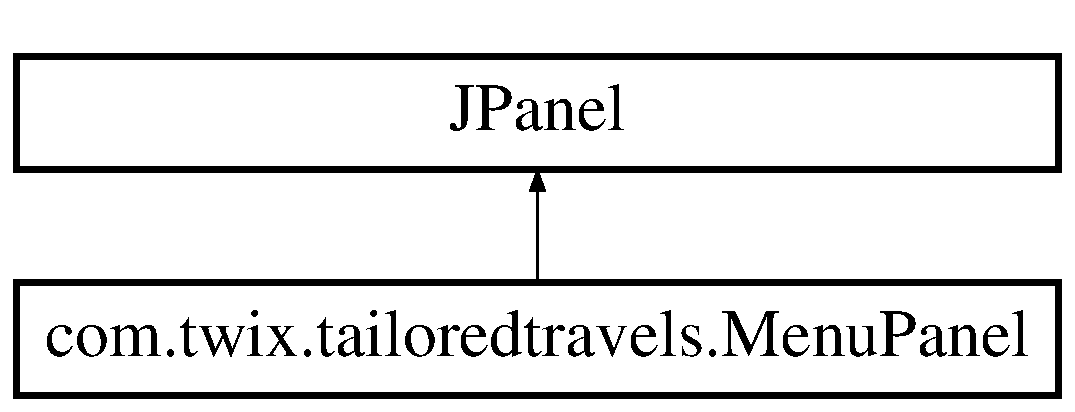
\includegraphics[height=2.000000cm]{classcom_1_1twix_1_1tailoredtravels_1_1_menu_panel}
\end{center}
\end{figure}
\subsection*{Public Member Functions}
\begin{DoxyCompactItemize}
\item 
\hyperlink{classcom_1_1twix_1_1tailoredtravels_1_1_menu_panel_aa85bfae72b9b9077e404b43b71789250}{Menu\-Panel} (\hyperlink{classcom_1_1twix_1_1tailoredtravels_1_1_database_manager}{Database\-Manager} dbm, String user, boolean admin)
\item 
void \hyperlink{classcom_1_1twix_1_1tailoredtravels_1_1_menu_panel_aaa1aefac37f56d3bfef741bd25634803}{add\-Components} ()
\item 
void \hyperlink{classcom_1_1twix_1_1tailoredtravels_1_1_menu_panel_a3f44b3bda0c13cd20e55712f05a9a37b}{update\-J\-List} ()
\end{DoxyCompactItemize}


\subsection{Detailed Description}


Definition at line 46 of file Menu\-Panel.\-java.



\subsection{Constructor \& Destructor Documentation}
\hypertarget{classcom_1_1twix_1_1tailoredtravels_1_1_menu_panel_aa85bfae72b9b9077e404b43b71789250}{\index{com\-::twix\-::tailoredtravels\-::\-Menu\-Panel@{com\-::twix\-::tailoredtravels\-::\-Menu\-Panel}!Menu\-Panel@{Menu\-Panel}}
\index{Menu\-Panel@{Menu\-Panel}!com::twix::tailoredtravels::MenuPanel@{com\-::twix\-::tailoredtravels\-::\-Menu\-Panel}}
\subsubsection[{Menu\-Panel}]{\setlength{\rightskip}{0pt plus 5cm}com.\-twix.\-tailoredtravels.\-Menu\-Panel.\-Menu\-Panel (
\begin{DoxyParamCaption}
\item[{{\bf Database\-Manager}}]{dbm, }
\item[{String}]{user, }
\item[{boolean}]{admin}
\end{DoxyParamCaption}
)}}\label{classcom_1_1twix_1_1tailoredtravels_1_1_menu_panel_aa85bfae72b9b9077e404b43b71789250}
Constructor for main menu


\begin{DoxyParams}{Parameters}
{\em dbm} & the database manager \\
\hline
{\em user} & the user's username \\
\hline
{\em admin} & whether or not the user is an administrator \\
\hline
\end{DoxyParams}


Definition at line 97 of file Menu\-Panel.\-java.



\subsection{Member Function Documentation}
\hypertarget{classcom_1_1twix_1_1tailoredtravels_1_1_menu_panel_aaa1aefac37f56d3bfef741bd25634803}{\index{com\-::twix\-::tailoredtravels\-::\-Menu\-Panel@{com\-::twix\-::tailoredtravels\-::\-Menu\-Panel}!add\-Components@{add\-Components}}
\index{add\-Components@{add\-Components}!com::twix::tailoredtravels::MenuPanel@{com\-::twix\-::tailoredtravels\-::\-Menu\-Panel}}
\subsubsection[{add\-Components}]{\setlength{\rightskip}{0pt plus 5cm}void com.\-twix.\-tailoredtravels.\-Menu\-Panel.\-add\-Components (
\begin{DoxyParamCaption}
{}
\end{DoxyParamCaption}
)}}\label{classcom_1_1twix_1_1tailoredtravels_1_1_menu_panel_aaa1aefac37f56d3bfef741bd25634803}
Add appropriate components to the main menu. 

Definition at line 226 of file Menu\-Panel.\-java.

\hypertarget{classcom_1_1twix_1_1tailoredtravels_1_1_menu_panel_a3f44b3bda0c13cd20e55712f05a9a37b}{\index{com\-::twix\-::tailoredtravels\-::\-Menu\-Panel@{com\-::twix\-::tailoredtravels\-::\-Menu\-Panel}!update\-J\-List@{update\-J\-List}}
\index{update\-J\-List@{update\-J\-List}!com::twix::tailoredtravels::MenuPanel@{com\-::twix\-::tailoredtravels\-::\-Menu\-Panel}}
\subsubsection[{update\-J\-List}]{\setlength{\rightskip}{0pt plus 5cm}void com.\-twix.\-tailoredtravels.\-Menu\-Panel.\-update\-J\-List (
\begin{DoxyParamCaption}
{}
\end{DoxyParamCaption}
)}}\label{classcom_1_1twix_1_1tailoredtravels_1_1_menu_panel_a3f44b3bda0c13cd20e55712f05a9a37b}
Update list of waypoints for changes with edits, adding and removing 

Definition at line 244 of file Menu\-Panel.\-java.



The documentation for this class was generated from the following file\-:\begin{DoxyCompactItemize}
\item 
C\-:/\-Users/\-Justin/workspace/\-Tailored Travels/src/com/twix/tailoredtravels/Menu\-Panel.\-java\end{DoxyCompactItemize}

\hypertarget{classcom_1_1twix_1_1tailoredtravels_1_1_progress_bar}{\section{com.\-twix.\-tailoredtravels.\-Progress\-Bar Class Reference}
\label{classcom_1_1twix_1_1tailoredtravels_1_1_progress_bar}\index{com.\-twix.\-tailoredtravels.\-Progress\-Bar@{com.\-twix.\-tailoredtravels.\-Progress\-Bar}}
}
Inheritance diagram for com.\-twix.\-tailoredtravels.\-Progress\-Bar\-:\begin{figure}[H]
\begin{center}
\leavevmode
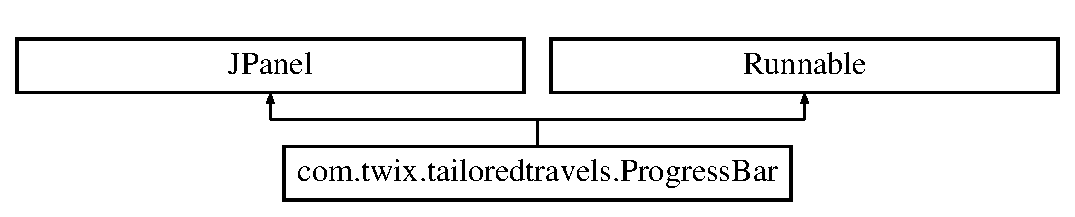
\includegraphics[height=2.000000cm]{classcom_1_1twix_1_1tailoredtravels_1_1_progress_bar}
\end{center}
\end{figure}
\subsection*{Public Member Functions}
\begin{DoxyCompactItemize}
\item 
\hypertarget{classcom_1_1twix_1_1tailoredtravels_1_1_progress_bar_a8802d9d9a03e351ab06e2aaab77e8667}{void {\bfseries run} ()}\label{classcom_1_1twix_1_1tailoredtravels_1_1_progress_bar_a8802d9d9a03e351ab06e2aaab77e8667}

\item 
\hypertarget{classcom_1_1twix_1_1tailoredtravels_1_1_progress_bar_a811166dd9c9e35124583d224f9c1b308}{void {\bfseries run\-Bar} ()}\label{classcom_1_1twix_1_1tailoredtravels_1_1_progress_bar_a811166dd9c9e35124583d224f9c1b308}

\item 
\hypertarget{classcom_1_1twix_1_1tailoredtravels_1_1_progress_bar_af3976bd1a762e92eba57524cf65fe400}{void {\bfseries set\-Start} (boolean start)}\label{classcom_1_1twix_1_1tailoredtravels_1_1_progress_bar_af3976bd1a762e92eba57524cf65fe400}

\end{DoxyCompactItemize}


\subsection{Detailed Description}


Definition at line 12 of file Progress\-Bar.\-java.



The documentation for this class was generated from the following file\-:\begin{DoxyCompactItemize}
\item 
C\-:/\-Users/\-Justin/workspace/\-Tailored Travels/src/com/twix/tailoredtravels/Progress\-Bar.\-java\end{DoxyCompactItemize}

\hypertarget{classcom_1_1twix_1_1tailoredtravels_1_1_waypoint}{\section{com.\-twix.\-tailoredtravels.\-Waypoint Class Reference}
\label{classcom_1_1twix_1_1tailoredtravels_1_1_waypoint}\index{com.\-twix.\-tailoredtravels.\-Waypoint@{com.\-twix.\-tailoredtravels.\-Waypoint}}
}
\subsection*{Public Member Functions}
\begin{DoxyCompactItemize}
\item 
\hyperlink{classcom_1_1twix_1_1tailoredtravels_1_1_waypoint_ac044cb6236cc8f91e403d5e397b0138c}{Waypoint} (String \-\_\-name, float \-\_\-lat, float \-\_\-long, String \-\_\-desc)
\item 
\hyperlink{classcom_1_1twix_1_1tailoredtravels_1_1_waypoint_a3cb2334fde8914ad02eca0daee98b052}{Waypoint} (float \-\_\-lat, float \-\_\-long)
\item 
\hyperlink{classcom_1_1twix_1_1tailoredtravels_1_1_waypoint_a6311fa930e1ebacee5795a7561f7d154}{Waypoint} ()
\item 
float \hyperlink{classcom_1_1twix_1_1tailoredtravels_1_1_waypoint_a0e9dfbf7825a6bc9494fe0ad5d28cf06}{get\-Longitude} ()
\item 
float \hyperlink{classcom_1_1twix_1_1tailoredtravels_1_1_waypoint_acd8b73a13740dcc01cfdf0f51afabc98}{get\-Latitude} ()
\item 
String \hyperlink{classcom_1_1twix_1_1tailoredtravels_1_1_waypoint_aa3e053c2012fd6c83ac266ebae053d41}{get\-Name} ()
\item 
String \hyperlink{classcom_1_1twix_1_1tailoredtravels_1_1_waypoint_a3d3b52f82622f22c603c06d1628fba4d}{get\-Description} ()
\item 
void \hyperlink{classcom_1_1twix_1_1tailoredtravels_1_1_waypoint_acde4707588dffddc9b270ac010ac3c49}{setw\-Name} (String w\-Name)
\item 
void \hyperlink{classcom_1_1twix_1_1tailoredtravels_1_1_waypoint_a3c4ea883b15c1f255d7debcefad30a3f}{setw\-Description} (String w\-Description)
\item 
void \hyperlink{classcom_1_1twix_1_1tailoredtravels_1_1_waypoint_a0a8ac77e3bbdcc661d84f221a890fa63}{setw\-Longitude} (float w\-Longitude)
\item 
void \hyperlink{classcom_1_1twix_1_1tailoredtravels_1_1_waypoint_aa5ff7b18588db74d9535a228106a2590}{setw\-Latitude} (float w\-Latitude)
\item 
double \hyperlink{classcom_1_1twix_1_1tailoredtravels_1_1_waypoint_ab533fb412000d0e8dd40ec688fcf5af1}{distance} (\hyperlink{classcom_1_1twix_1_1tailoredtravels_1_1_waypoint}{Waypoint} other)
\item 
boolean \hyperlink{classcom_1_1twix_1_1tailoredtravels_1_1_waypoint_a6108a1c61439902f3c31aa4b4509069d}{equals} (\hyperlink{classcom_1_1twix_1_1tailoredtravels_1_1_waypoint}{Waypoint} other)
\item 
String \hyperlink{classcom_1_1twix_1_1tailoredtravels_1_1_waypoint_a874ca189dbecb33168c5068afbf82aa7}{to\-String} ()
\item 
String \hyperlink{classcom_1_1twix_1_1tailoredtravels_1_1_waypoint_a55b51e30c9195587908b5b3115e7c482}{print\-Database} ()
\end{DoxyCompactItemize}


\subsection{Detailed Description}
A class that acts as the template for K\-M\-L objects correlating to locations.

\begin{DoxyAuthor}{Author}
Stephen Moore \& Justin Tavares with distance function by Mariama Barr-\/\-Dallas, Michael Tang 
\end{DoxyAuthor}


\subsection{Constructor \& Destructor Documentation}
\hypertarget{classcom_1_1twix_1_1tailoredtravels_1_1_waypoint_ac044cb6236cc8f91e403d5e397b0138c}{\index{com\-::twix\-::tailoredtravels\-::\-Waypoint@{com\-::twix\-::tailoredtravels\-::\-Waypoint}!Waypoint@{Waypoint}}
\index{Waypoint@{Waypoint}!com::twix::tailoredtravels::Waypoint@{com\-::twix\-::tailoredtravels\-::\-Waypoint}}
\subsubsection[{Waypoint}]{\setlength{\rightskip}{0pt plus 5cm}com.\-twix.\-tailoredtravels.\-Waypoint.\-Waypoint (
\begin{DoxyParamCaption}
\item[{String}]{\-\_\-name, }
\item[{float}]{\-\_\-lat, }
\item[{float}]{\-\_\-long, }
\item[{String}]{\-\_\-desc}
\end{DoxyParamCaption}
)}}\label{classcom_1_1twix_1_1tailoredtravels_1_1_waypoint_ac044cb6236cc8f91e403d5e397b0138c}
Float constructor, creates waypoint with name, latitude, longitude, description given in input


\begin{DoxyParams}{Parameters}
{\em \-\_\-name} & name of waypoint \\
\hline
{\em \-\_\-lat} & latitude of waypoint \\
\hline
{\em \-\_\-long} & longitude of waypoint \\
\hline
{\em \-\_\-desc} & description of waypoint \\
\hline
\end{DoxyParams}
\hypertarget{classcom_1_1twix_1_1tailoredtravels_1_1_waypoint_a3cb2334fde8914ad02eca0daee98b052}{\index{com\-::twix\-::tailoredtravels\-::\-Waypoint@{com\-::twix\-::tailoredtravels\-::\-Waypoint}!Waypoint@{Waypoint}}
\index{Waypoint@{Waypoint}!com::twix::tailoredtravels::Waypoint@{com\-::twix\-::tailoredtravels\-::\-Waypoint}}
\subsubsection[{Waypoint}]{\setlength{\rightskip}{0pt plus 5cm}com.\-twix.\-tailoredtravels.\-Waypoint.\-Waypoint (
\begin{DoxyParamCaption}
\item[{float}]{\-\_\-lat, }
\item[{float}]{\-\_\-long}
\end{DoxyParamCaption}
)}}\label{classcom_1_1twix_1_1tailoredtravels_1_1_waypoint_a3cb2334fde8914ad02eca0daee98b052}
No name/desc constructor for \hyperlink{classcom_1_1twix_1_1tailoredtravels_1_1_waypoint}{Waypoint}, creates a nameless waypoint with given latitude/longitude


\begin{DoxyParams}{Parameters}
{\em \-\_\-lat} & latitude of waypoint \\
\hline
{\em \-\_\-long} & longitude of waypoint \\
\hline
\end{DoxyParams}
\hypertarget{classcom_1_1twix_1_1tailoredtravels_1_1_waypoint_a6311fa930e1ebacee5795a7561f7d154}{\index{com\-::twix\-::tailoredtravels\-::\-Waypoint@{com\-::twix\-::tailoredtravels\-::\-Waypoint}!Waypoint@{Waypoint}}
\index{Waypoint@{Waypoint}!com::twix::tailoredtravels::Waypoint@{com\-::twix\-::tailoredtravels\-::\-Waypoint}}
\subsubsection[{Waypoint}]{\setlength{\rightskip}{0pt plus 5cm}com.\-twix.\-tailoredtravels.\-Waypoint.\-Waypoint (
\begin{DoxyParamCaption}
{}
\end{DoxyParamCaption}
)}}\label{classcom_1_1twix_1_1tailoredtravels_1_1_waypoint_a6311fa930e1ebacee5795a7561f7d154}
Noarg constructor 

\subsection{Member Function Documentation}
\hypertarget{classcom_1_1twix_1_1tailoredtravels_1_1_waypoint_ab533fb412000d0e8dd40ec688fcf5af1}{\index{com\-::twix\-::tailoredtravels\-::\-Waypoint@{com\-::twix\-::tailoredtravels\-::\-Waypoint}!distance@{distance}}
\index{distance@{distance}!com::twix::tailoredtravels::Waypoint@{com\-::twix\-::tailoredtravels\-::\-Waypoint}}
\subsubsection[{distance}]{\setlength{\rightskip}{0pt plus 5cm}double com.\-twix.\-tailoredtravels.\-Waypoint.\-distance (
\begin{DoxyParamCaption}
\item[{{\bf Waypoint}}]{other}
\end{DoxyParamCaption}
)}}\label{classcom_1_1twix_1_1tailoredtravels_1_1_waypoint_ab533fb412000d0e8dd40ec688fcf5af1}
Calculates the distance between 2 coordinates in miles Equation for calculation\-: dlon = lon2 -\/ lon1 dlat = lat2 -\/ lat1 a = (sin(dlat/2))$^\wedge$2 + cos(lat1) $\ast$ cos(lat2) $\ast$ (sin(dlon/2))$^\wedge$2 c = 2 $\ast$ atan2( sqrt(a), sqrt(1-\/a) ) d = R $\ast$ c (where R is the radius of the Earth)


\begin{DoxyParams}{Parameters}
{\em other} & other waypoint for distance calculation\\
\hline
\end{DoxyParams}
\begin{DoxyReturn}{Returns}
double containing distance between 2 coordinates 
\end{DoxyReturn}
\hypertarget{classcom_1_1twix_1_1tailoredtravels_1_1_waypoint_a6108a1c61439902f3c31aa4b4509069d}{\index{com\-::twix\-::tailoredtravels\-::\-Waypoint@{com\-::twix\-::tailoredtravels\-::\-Waypoint}!equals@{equals}}
\index{equals@{equals}!com::twix::tailoredtravels::Waypoint@{com\-::twix\-::tailoredtravels\-::\-Waypoint}}
\subsubsection[{equals}]{\setlength{\rightskip}{0pt plus 5cm}boolean com.\-twix.\-tailoredtravels.\-Waypoint.\-equals (
\begin{DoxyParamCaption}
\item[{{\bf Waypoint}}]{other}
\end{DoxyParamCaption}
)}}\label{classcom_1_1twix_1_1tailoredtravels_1_1_waypoint_a6108a1c61439902f3c31aa4b4509069d}
Determines if this waypoint is the same as a given waypoint


\begin{DoxyParams}{Parameters}
{\em other} & other waypoint for distance calculation \\
\hline
\end{DoxyParams}
\begin{DoxyReturn}{Returns}
true if waypoints are the same, false otherwise 
\end{DoxyReturn}
\hypertarget{classcom_1_1twix_1_1tailoredtravels_1_1_waypoint_a3d3b52f82622f22c603c06d1628fba4d}{\index{com\-::twix\-::tailoredtravels\-::\-Waypoint@{com\-::twix\-::tailoredtravels\-::\-Waypoint}!get\-Description@{get\-Description}}
\index{get\-Description@{get\-Description}!com::twix::tailoredtravels::Waypoint@{com\-::twix\-::tailoredtravels\-::\-Waypoint}}
\subsubsection[{get\-Description}]{\setlength{\rightskip}{0pt plus 5cm}String com.\-twix.\-tailoredtravels.\-Waypoint.\-get\-Description (
\begin{DoxyParamCaption}
{}
\end{DoxyParamCaption}
)}}\label{classcom_1_1twix_1_1tailoredtravels_1_1_waypoint_a3d3b52f82622f22c603c06d1628fba4d}
get\-Description \begin{DoxyReturn}{Returns}
w\-Description 
\end{DoxyReturn}
\hypertarget{classcom_1_1twix_1_1tailoredtravels_1_1_waypoint_acd8b73a13740dcc01cfdf0f51afabc98}{\index{com\-::twix\-::tailoredtravels\-::\-Waypoint@{com\-::twix\-::tailoredtravels\-::\-Waypoint}!get\-Latitude@{get\-Latitude}}
\index{get\-Latitude@{get\-Latitude}!com::twix::tailoredtravels::Waypoint@{com\-::twix\-::tailoredtravels\-::\-Waypoint}}
\subsubsection[{get\-Latitude}]{\setlength{\rightskip}{0pt plus 5cm}float com.\-twix.\-tailoredtravels.\-Waypoint.\-get\-Latitude (
\begin{DoxyParamCaption}
{}
\end{DoxyParamCaption}
)}}\label{classcom_1_1twix_1_1tailoredtravels_1_1_waypoint_acd8b73a13740dcc01cfdf0f51afabc98}
get\-Latitude \begin{DoxyReturn}{Returns}
w\-Latitude 
\end{DoxyReturn}
\hypertarget{classcom_1_1twix_1_1tailoredtravels_1_1_waypoint_a0e9dfbf7825a6bc9494fe0ad5d28cf06}{\index{com\-::twix\-::tailoredtravels\-::\-Waypoint@{com\-::twix\-::tailoredtravels\-::\-Waypoint}!get\-Longitude@{get\-Longitude}}
\index{get\-Longitude@{get\-Longitude}!com::twix::tailoredtravels::Waypoint@{com\-::twix\-::tailoredtravels\-::\-Waypoint}}
\subsubsection[{get\-Longitude}]{\setlength{\rightskip}{0pt plus 5cm}float com.\-twix.\-tailoredtravels.\-Waypoint.\-get\-Longitude (
\begin{DoxyParamCaption}
{}
\end{DoxyParamCaption}
)}}\label{classcom_1_1twix_1_1tailoredtravels_1_1_waypoint_a0e9dfbf7825a6bc9494fe0ad5d28cf06}
get\-Longitude \begin{DoxyReturn}{Returns}
w\-Longitude 
\end{DoxyReturn}
\hypertarget{classcom_1_1twix_1_1tailoredtravels_1_1_waypoint_aa3e053c2012fd6c83ac266ebae053d41}{\index{com\-::twix\-::tailoredtravels\-::\-Waypoint@{com\-::twix\-::tailoredtravels\-::\-Waypoint}!get\-Name@{get\-Name}}
\index{get\-Name@{get\-Name}!com::twix::tailoredtravels::Waypoint@{com\-::twix\-::tailoredtravels\-::\-Waypoint}}
\subsubsection[{get\-Name}]{\setlength{\rightskip}{0pt plus 5cm}String com.\-twix.\-tailoredtravels.\-Waypoint.\-get\-Name (
\begin{DoxyParamCaption}
{}
\end{DoxyParamCaption}
)}}\label{classcom_1_1twix_1_1tailoredtravels_1_1_waypoint_aa3e053c2012fd6c83ac266ebae053d41}
get\-Name \begin{DoxyReturn}{Returns}
w\-Name 
\end{DoxyReturn}
\hypertarget{classcom_1_1twix_1_1tailoredtravels_1_1_waypoint_a55b51e30c9195587908b5b3115e7c482}{\index{com\-::twix\-::tailoredtravels\-::\-Waypoint@{com\-::twix\-::tailoredtravels\-::\-Waypoint}!print\-Database@{print\-Database}}
\index{print\-Database@{print\-Database}!com::twix::tailoredtravels::Waypoint@{com\-::twix\-::tailoredtravels\-::\-Waypoint}}
\subsubsection[{print\-Database}]{\setlength{\rightskip}{0pt plus 5cm}String com.\-twix.\-tailoredtravels.\-Waypoint.\-print\-Database (
\begin{DoxyParamCaption}
{}
\end{DoxyParamCaption}
)}}\label{classcom_1_1twix_1_1tailoredtravels_1_1_waypoint_a55b51e30c9195587908b5b3115e7c482}
\hypertarget{classcom_1_1twix_1_1tailoredtravels_1_1_waypoint_a3c4ea883b15c1f255d7debcefad30a3f}{\index{com\-::twix\-::tailoredtravels\-::\-Waypoint@{com\-::twix\-::tailoredtravels\-::\-Waypoint}!setw\-Description@{setw\-Description}}
\index{setw\-Description@{setw\-Description}!com::twix::tailoredtravels::Waypoint@{com\-::twix\-::tailoredtravels\-::\-Waypoint}}
\subsubsection[{setw\-Description}]{\setlength{\rightskip}{0pt plus 5cm}void com.\-twix.\-tailoredtravels.\-Waypoint.\-setw\-Description (
\begin{DoxyParamCaption}
\item[{String}]{w\-Description}
\end{DoxyParamCaption}
)}}\label{classcom_1_1twix_1_1tailoredtravels_1_1_waypoint_a3c4ea883b15c1f255d7debcefad30a3f}
setw\-Description 
\begin{DoxyParams}{Parameters}
{\em w\-Description} & new description \\
\hline
\end{DoxyParams}
\hypertarget{classcom_1_1twix_1_1tailoredtravels_1_1_waypoint_aa5ff7b18588db74d9535a228106a2590}{\index{com\-::twix\-::tailoredtravels\-::\-Waypoint@{com\-::twix\-::tailoredtravels\-::\-Waypoint}!setw\-Latitude@{setw\-Latitude}}
\index{setw\-Latitude@{setw\-Latitude}!com::twix::tailoredtravels::Waypoint@{com\-::twix\-::tailoredtravels\-::\-Waypoint}}
\subsubsection[{setw\-Latitude}]{\setlength{\rightskip}{0pt plus 5cm}void com.\-twix.\-tailoredtravels.\-Waypoint.\-setw\-Latitude (
\begin{DoxyParamCaption}
\item[{float}]{w\-Latitude}
\end{DoxyParamCaption}
)}}\label{classcom_1_1twix_1_1tailoredtravels_1_1_waypoint_aa5ff7b18588db74d9535a228106a2590}
setw\-Latitude 
\begin{DoxyParams}{Parameters}
{\em w\-Latitude} & new latitude \\
\hline
\end{DoxyParams}
\hypertarget{classcom_1_1twix_1_1tailoredtravels_1_1_waypoint_a0a8ac77e3bbdcc661d84f221a890fa63}{\index{com\-::twix\-::tailoredtravels\-::\-Waypoint@{com\-::twix\-::tailoredtravels\-::\-Waypoint}!setw\-Longitude@{setw\-Longitude}}
\index{setw\-Longitude@{setw\-Longitude}!com::twix::tailoredtravels::Waypoint@{com\-::twix\-::tailoredtravels\-::\-Waypoint}}
\subsubsection[{setw\-Longitude}]{\setlength{\rightskip}{0pt plus 5cm}void com.\-twix.\-tailoredtravels.\-Waypoint.\-setw\-Longitude (
\begin{DoxyParamCaption}
\item[{float}]{w\-Longitude}
\end{DoxyParamCaption}
)}}\label{classcom_1_1twix_1_1tailoredtravels_1_1_waypoint_a0a8ac77e3bbdcc661d84f221a890fa63}
setw\-Longitude 
\begin{DoxyParams}{Parameters}
{\em w\-Longitude} & new longitude \\
\hline
\end{DoxyParams}
\hypertarget{classcom_1_1twix_1_1tailoredtravels_1_1_waypoint_acde4707588dffddc9b270ac010ac3c49}{\index{com\-::twix\-::tailoredtravels\-::\-Waypoint@{com\-::twix\-::tailoredtravels\-::\-Waypoint}!setw\-Name@{setw\-Name}}
\index{setw\-Name@{setw\-Name}!com::twix::tailoredtravels::Waypoint@{com\-::twix\-::tailoredtravels\-::\-Waypoint}}
\subsubsection[{setw\-Name}]{\setlength{\rightskip}{0pt plus 5cm}void com.\-twix.\-tailoredtravels.\-Waypoint.\-setw\-Name (
\begin{DoxyParamCaption}
\item[{String}]{w\-Name}
\end{DoxyParamCaption}
)}}\label{classcom_1_1twix_1_1tailoredtravels_1_1_waypoint_acde4707588dffddc9b270ac010ac3c49}
setw\-Name 
\begin{DoxyParams}{Parameters}
{\em w\-Name} & new name \\
\hline
\end{DoxyParams}
\hypertarget{classcom_1_1twix_1_1tailoredtravels_1_1_waypoint_a874ca189dbecb33168c5068afbf82aa7}{\index{com\-::twix\-::tailoredtravels\-::\-Waypoint@{com\-::twix\-::tailoredtravels\-::\-Waypoint}!to\-String@{to\-String}}
\index{to\-String@{to\-String}!com::twix::tailoredtravels::Waypoint@{com\-::twix\-::tailoredtravels\-::\-Waypoint}}
\subsubsection[{to\-String}]{\setlength{\rightskip}{0pt plus 5cm}String com.\-twix.\-tailoredtravels.\-Waypoint.\-to\-String (
\begin{DoxyParamCaption}
{}
\end{DoxyParamCaption}
)}}\label{classcom_1_1twix_1_1tailoredtravels_1_1_waypoint_a874ca189dbecb33168c5068afbf82aa7}
to\-String -\/ returns w\-Name, w\-Latitude\-:w\-Longitude, w\-Description 

The documentation for this class was generated from the following file\-:\begin{DoxyCompactItemize}
\item 
C\-:/\-Users/\-Justin/workspace/\-Tailored Travels/src/com/twix/tailoredtravels/\hyperlink{_waypoint_8java}{Waypoint.\-java}\end{DoxyCompactItemize}

\chapter{File Documentation}
\hypertarget{_init_database_8java}{\section{C\-:/\-Users/\-Justin/workspace/\-Tailored Travels/src/com/twix/init/\-Init\-Database.java File Reference}
\label{_init_database_8java}\index{C\-:/\-Users/\-Justin/workspace/\-Tailored Travels/src/com/twix/init/\-Init\-Database.\-java@{C\-:/\-Users/\-Justin/workspace/\-Tailored Travels/src/com/twix/init/\-Init\-Database.\-java}}
}
\subsection*{Classes}
\begin{DoxyCompactItemize}
\item 
class \hyperlink{classcom_1_1twix_1_1init_1_1_init_database}{com.\-twix.\-init.\-Init\-Database}
\end{DoxyCompactItemize}
\subsection*{Packages}
\begin{DoxyCompactItemize}
\item 
package \hyperlink{namespacecom_1_1twix_1_1init}{com.\-twix.\-init}
\end{DoxyCompactItemize}

\hypertarget{_client_8java}{\section{C\-:/\-Users/\-Justin/workspace/\-Tailored Travels/src/com/twix/tailoredtravels/\-Client.java File Reference}
\label{_client_8java}\index{C\-:/\-Users/\-Justin/workspace/\-Tailored Travels/src/com/twix/tailoredtravels/\-Client.\-java@{C\-:/\-Users/\-Justin/workspace/\-Tailored Travels/src/com/twix/tailoredtravels/\-Client.\-java}}
}
\subsection*{Classes}
\begin{DoxyCompactItemize}
\item 
class \hyperlink{classcom_1_1twix_1_1tailoredtravels_1_1_client}{com.\-twix.\-tailoredtravels.\-Client}
\end{DoxyCompactItemize}
\subsection*{Packages}
\begin{DoxyCompactItemize}
\item 
package \hyperlink{namespacecom_1_1twix_1_1tailoredtravels}{com.\-twix.\-tailoredtravels}
\end{DoxyCompactItemize}

\hypertarget{_database_manager_8java}{\section{C\-:/\-Users/\-Justin/workspace/\-Tailored Travels/src/com/twix/tailoredtravels/\-Database\-Manager.java File Reference}
\label{_database_manager_8java}\index{C\-:/\-Users/\-Justin/workspace/\-Tailored Travels/src/com/twix/tailoredtravels/\-Database\-Manager.\-java@{C\-:/\-Users/\-Justin/workspace/\-Tailored Travels/src/com/twix/tailoredtravels/\-Database\-Manager.\-java}}
}
\subsection*{Classes}
\begin{DoxyCompactItemize}
\item 
class \hyperlink{classcom_1_1twix_1_1tailoredtravels_1_1_database_manager}{com.\-twix.\-tailoredtravels.\-Database\-Manager}
\end{DoxyCompactItemize}
\subsection*{Packages}
\begin{DoxyCompactItemize}
\item 
package \hyperlink{namespacecom_1_1twix_1_1tailoredtravels}{com.\-twix.\-tailoredtravels}
\end{DoxyCompactItemize}

\hypertarget{_dist_calc_driver_8java}{\section{C\-:/\-Users/\-Justin/workspace/\-Tailored Travels/src/com/twix/tailoredtravels/\-Dist\-Calc\-Driver.java File Reference}
\label{_dist_calc_driver_8java}\index{C\-:/\-Users/\-Justin/workspace/\-Tailored Travels/src/com/twix/tailoredtravels/\-Dist\-Calc\-Driver.\-java@{C\-:/\-Users/\-Justin/workspace/\-Tailored Travels/src/com/twix/tailoredtravels/\-Dist\-Calc\-Driver.\-java}}
}
\subsection*{Classes}
\begin{DoxyCompactItemize}
\item 
class \hyperlink{classcom_1_1twix_1_1tailoredtravels_1_1_dist_calc_driver}{com.\-twix.\-tailoredtravels.\-Dist\-Calc\-Driver}
\end{DoxyCompactItemize}
\subsection*{Packages}
\begin{DoxyCompactItemize}
\item 
package \hyperlink{namespacecom_1_1twix_1_1tailoredtravels}{com.\-twix.\-tailoredtravels}
\end{DoxyCompactItemize}

\hypertarget{_google_earth_manager_8java}{\section{C\-:/\-Users/\-Justin/workspace/\-Tailored Travels/src/com/twix/tailoredtravels/\-Google\-Earth\-Manager.java File Reference}
\label{_google_earth_manager_8java}\index{C\-:/\-Users/\-Justin/workspace/\-Tailored Travels/src/com/twix/tailoredtravels/\-Google\-Earth\-Manager.\-java@{C\-:/\-Users/\-Justin/workspace/\-Tailored Travels/src/com/twix/tailoredtravels/\-Google\-Earth\-Manager.\-java}}
}
\subsection*{Classes}
\begin{DoxyCompactItemize}
\item 
class \hyperlink{classcom_1_1twix_1_1tailoredtravels_1_1_google_earth_manager}{com.\-twix.\-tailoredtravels.\-Google\-Earth\-Manager}
\end{DoxyCompactItemize}
\subsection*{Packages}
\begin{DoxyCompactItemize}
\item 
package \hyperlink{namespacecom_1_1twix_1_1tailoredtravels}{com.\-twix.\-tailoredtravels}
\end{DoxyCompactItemize}

\hypertarget{_google_earth_path_8java}{\section{C\-:/\-Users/\-Justin/workspace/\-Tailored Travels/src/com/twix/tailoredtravels/\-Google\-Earth\-Path.java File Reference}
\label{_google_earth_path_8java}\index{C\-:/\-Users/\-Justin/workspace/\-Tailored Travels/src/com/twix/tailoredtravels/\-Google\-Earth\-Path.\-java@{C\-:/\-Users/\-Justin/workspace/\-Tailored Travels/src/com/twix/tailoredtravels/\-Google\-Earth\-Path.\-java}}
}
\subsection*{Classes}
\begin{DoxyCompactItemize}
\item 
class \hyperlink{classcom_1_1twix_1_1tailoredtravels_1_1_google_earth_path}{com.\-twix.\-tailoredtravels.\-Google\-Earth\-Path}
\end{DoxyCompactItemize}
\subsection*{Packages}
\begin{DoxyCompactItemize}
\item 
package \hyperlink{namespacecom_1_1twix_1_1tailoredtravels}{com.\-twix.\-tailoredtravels}
\end{DoxyCompactItemize}

\hypertarget{_lat_long_pair_8java}{\section{C\-:/\-Users/\-Justin/workspace/\-Tailored Travels/src/com/twix/tailoredtravels/\-Lat\-Long\-Pair.java File Reference}
\label{_lat_long_pair_8java}\index{C\-:/\-Users/\-Justin/workspace/\-Tailored Travels/src/com/twix/tailoredtravels/\-Lat\-Long\-Pair.\-java@{C\-:/\-Users/\-Justin/workspace/\-Tailored Travels/src/com/twix/tailoredtravels/\-Lat\-Long\-Pair.\-java}}
}
\subsection*{Classes}
\begin{DoxyCompactItemize}
\item 
class \hyperlink{classcom_1_1twix_1_1tailoredtravels_1_1_lat_long_pair}{com.\-twix.\-tailoredtravels.\-Lat\-Long\-Pair}
\end{DoxyCompactItemize}
\subsection*{Packages}
\begin{DoxyCompactItemize}
\item 
package \hyperlink{namespacecom_1_1twix_1_1tailoredtravels}{com.\-twix.\-tailoredtravels}
\end{DoxyCompactItemize}

\hypertarget{_menu_panel_8java}{\section{C\-:/\-Users/\-Justin/workspace/\-Tailored Travels/src/com/twix/tailoredtravels/\-Menu\-Panel.java File Reference}
\label{_menu_panel_8java}\index{C\-:/\-Users/\-Justin/workspace/\-Tailored Travels/src/com/twix/tailoredtravels/\-Menu\-Panel.\-java@{C\-:/\-Users/\-Justin/workspace/\-Tailored Travels/src/com/twix/tailoredtravels/\-Menu\-Panel.\-java}}
}
\subsection*{Classes}
\begin{DoxyCompactItemize}
\item 
class \hyperlink{classcom_1_1twix_1_1tailoredtravels_1_1_menu_panel}{com.\-twix.\-tailoredtravels.\-Menu\-Panel}
\end{DoxyCompactItemize}
\subsection*{Packages}
\begin{DoxyCompactItemize}
\item 
package \hyperlink{namespacecom_1_1twix_1_1tailoredtravels}{com.\-twix.\-tailoredtravels}
\end{DoxyCompactItemize}

\hypertarget{_progress_bar_8java}{\section{C\-:/\-Users/\-Justin/workspace/\-Tailored Travels/src/com/twix/tailoredtravels/\-Progress\-Bar.java File Reference}
\label{_progress_bar_8java}\index{C\-:/\-Users/\-Justin/workspace/\-Tailored Travels/src/com/twix/tailoredtravels/\-Progress\-Bar.\-java@{C\-:/\-Users/\-Justin/workspace/\-Tailored Travels/src/com/twix/tailoredtravels/\-Progress\-Bar.\-java}}
}
\subsection*{Classes}
\begin{DoxyCompactItemize}
\item 
class \hyperlink{classcom_1_1twix_1_1tailoredtravels_1_1_progress_bar}{com.\-twix.\-tailoredtravels.\-Progress\-Bar}
\end{DoxyCompactItemize}
\subsection*{Packages}
\begin{DoxyCompactItemize}
\item 
package \hyperlink{namespacecom_1_1twix_1_1tailoredtravels}{com.\-twix.\-tailoredtravels}
\end{DoxyCompactItemize}

\hypertarget{_waypoint_8java}{\section{C\-:/\-Users/\-Justin/workspace/\-Tailored Travels/src/com/twix/tailoredtravels/\-Waypoint.java File Reference}
\label{_waypoint_8java}\index{C\-:/\-Users/\-Justin/workspace/\-Tailored Travels/src/com/twix/tailoredtravels/\-Waypoint.\-java@{C\-:/\-Users/\-Justin/workspace/\-Tailored Travels/src/com/twix/tailoredtravels/\-Waypoint.\-java}}
}
\subsection*{Classes}
\begin{DoxyCompactItemize}
\item 
class \hyperlink{classcom_1_1twix_1_1tailoredtravels_1_1_waypoint}{com.\-twix.\-tailoredtravels.\-Waypoint}
\end{DoxyCompactItemize}
\subsection*{Packages}
\begin{DoxyCompactItemize}
\item 
package \hyperlink{namespacecom_1_1twix_1_1tailoredtravels}{com.\-twix.\-tailoredtravels}
\end{DoxyCompactItemize}

%--- End generated contents ---

% Index
\newpage
\phantomsection
\addcontentsline{toc}{part}{Index}
\printindex

\end{document}
